\documentclass[a4paper, twoside, 11pt]{scrreprt}

% !TEX root = Protokoll.tex
%Encoding
\usepackage[utf8]{inputenc}

%Formatierung Ränder (Optional)
\usepackage[left=2cm,right=2cm,top=2.3cm,bottom=2.3cm,includeheadfoot]{geometry}

%Spracheinstellung
\usepackage[english]{babel}
\usepackage{setspace}
\onehalfspacing
%\addto\captionsngerman{
%	\renewcommand{\figurename}{Abb.}
%	\renewcommand{\tablename}{Tab.}
%}

%Glaettung von Text
\usepackage{lmodern}

%Font-Encoding 
\usepackage[T1]{fontenc} 

%Tabellen und Grafiken
\usepackage{graphicx}
\usepackage{tabularx}
\setlength{\tabcolsep}{18pt}%space between text and left/right border
\usepackage{dcolumn}
\usepackage{multicol}
\usepackage{float}
\usepackage{floatflt}
\usepackage{here}
\usepackage{blindtext}
\newcolumntype{.}{D{.}{.}{7}}
\usepackage{wrapfig}
\usepackage{bigstrut}

\usepackage{subfig}

%\usepackage{subfigure}
\usepackage{here}

%Ueberschrift mit Serifen (nur Inhaltsverzeichnis)
\setkomafont{sectioning}{\normalfont\bfseries}

%Caption
\usepackage{caption}

%Mathe, Physik und Chemiepakete
\usepackage{amsfonts,amsmath,amssymb}
\usepackage[version=3]{mhchem}

%Units/Fraction
\usepackage[output-decimal-marker={.}, per-mode=fraction]{siunitx}
\usepackage{icomma}

%Nummerierung Gleichungen bei mehreren Kapiteln
\numberwithin{equation}{section}
\numberwithin{figure}{section}
\numberwithin{table}{section}

%Sonstiges
\usepackage{geometry}
\geometry{verbose,a4paper,tmargin=25mm,bmargin=25mm,lmargin=15mm,rmargin=20mm}
\usepackage{amsfonts}
\usepackage{amssymb}
\usepackage{latexsym}
\usepackage{texdraw}
\usepackage[T1]{fontenc}
\usepackage[breaklinks,pdfborder={0 0 0}]{hyperref}
\usepackage{url}
\usepackage{pgf}
\usepackage{tikz}
\usetikzlibrary{fit}

%Definierte Wortsilbentrennung
\hyphenation{Test}

%Bilder Ordner
\graphicspath{{plots/}}

%Titel
\title{Dokumenttitel}
\author{Autor}
\usepackage[headsepline]{scrpage2}
\pagestyle{scrheadings}
\clearscrheadfoot
\ihead{Wilkin Woehle}
\ofoot{\pagemark}
\ohead{\headmark}
\automark{section}

%Bibliography
%\usepackage{bibgerm}
\usepackage[backend=biber, style = phys,maxnames=4,clearlang=true,doi=false]{biblatex}
%\DeclareRedundantLanguages{english,german,french,en,de}{english,german,french,en,de}
\addbibresource{bib/library.bib}

\defbibfilter{papers}{
	type=article or
	type=inproceedings or
	type=incollection
} 


%Ueberschriften formatieren
\addtokomafont{title}{\normalfont\bfseries}
\addtokomafont{section}{\normalfont\bfseries\Large}
\addtokomafont{subsection}{\normalfont\bfseries\large}
\addtokomafont{subsubsection}{\normalfont\bfseries\normalsize}
\addtokomafont{paragraph}{\normalfont\bfseries\normalsize}


% Abstand nach math-Umgebungen
\setlength\abovedisplayshortskip{0pt}
\setlength\belowdisplayshortskip{0pt}
\setlength\abovedisplayskip{0pt}
\setlength\belowdisplayskip{0pt}

%Neu
\setlength{\parindent}{0pt}




% !TEX root = Protokoll.tex


%Namen Physiker
\newcommand{\Snellius}{\textnormal{\textsc{Snellius}} }
\newcommand{\Bohr}{\textnormal{\textsc{Bohr}} }
\newcommand{\Pickering}{\textnormal{\textsc{Pickering}} }
\newcommand{\Balmer}{\textnormal{\textsc{Balmer}} }
\newcommand{\Planck}{\textnormal{\textsc{Planck}} }
\newcommand{\Einstein}{\textnormal{\textsc{Einstein}} }
\newcommand{\Rydberg}{\textnormal{\textsc{Rydberg}} }
\newcommand{\Gauss}{\textnormal{\textsc{Gauß}} }
\newcommand{\Heisenberg}{\textnormal{\textsc{Heisenberg}} }
\newcommand{\Parseval}{\textnormal{\textsc{Parseval}} }
\newcommand{\Schroedinger}{\textnormal{\textsc{Schrödinger}} }
\newcommand{\Hamilton}{\textnormal{\textsc{Hamilton}} }
\newcommand{\Doppler}{\textnormal{\textsc{Doppler}} }
\newcommand{\Zeeman}{\textnormal{\textsc{Zeeman}} }
\newcommand{\FabryPerot}{\textnormal{\textsc{Fabry-Pérot}} }
\newcommand{\BiotSavart}{\textnormal{\textsc{Biot-Savart}} }
\newcommand{\Lande}{\textnormal{\textsc{Landé}} }
\newcommand{\Lorentz}{\textnormal{\textsc{Lorentz}} }
\newcommand{\Maxwell}{\textnormal{\textsc{Maxwell}} }
\newcommand{\CG}{\textnormal{\textsc{Clebsch-Gordon}} }
\newcommand{\Tesla}{\textnormal{\textsc{Tesla}} }


%Neue Komandos:
\newcommand{\todo}[1]{\textcolor{red}{#1}}
\newcommand{\newText}[1]{\textcolor{purple}{#1}}

\newcommand{\al}[1]{\begin{align}
	#1
	\end{align}}
\newcommand{\ali}[1]{\begin{align*}
	#1
	\end{align*}}
\newcommand{\inv}[1]{\frac{1}{#1}}
\newcommand{\itbf}[1]{\textit{\textbf{#1}}}
\renewcommand{\it}[1]{\textit{#1}}
\renewcommand{\sc}[1]{\textsc{#1}}
\renewcommand{\d}{\mathrm{d}}



%88888888888888888888888888888888888888888888888888888888888888888888888888
\begin{document}
	%set language
	\selectlanguage{english}
	
	%sections
	\renewcommand{\subsectionautorefname}{section\negthinspace}
	\renewcommand{\subsubsectionautorefname}{section\negthinspace}	\renewcommand{\figureautorefname}{fig.\negthinspace}
	\renewcommand{\tableautorefname}{tab.\negthinspace}
	\renewcommand{\equationautorefname}{eq.\negthinspace}
	
	
	\newcommand{\vtitle}{Nucleation and Crystallization of the Metastable Hard Sphere Fluid}
	\newcommand{\vinstitute}{Research group for complex systems and soft matter}
	\newcommand{\vsupervision}{Prof. Dr. Tanja Schilling}
	\newcommand{\vauthor}{Wilkin Wöhler}

	
	
	\newcommand{\presummary}{Nucleation and cluster development in the metastable hard sphere fluid are studied in this thesis. To this purpose an event driven molecular dynamcis simulation code is written and thouroughly tested by measuring well known quantities like diffusion coefficients or radial distribution functions at various packing fractions. Its performance is well suited for systems of about one million particles enabling the measurement of cluster growth rates and shape descriptors for clusters with sizes up to a hundred thousand particles without significant spatial influence of the cluster on to itself due to the periodic boundary conditions.\\ 
During the cluster growth a constant attachment rate to the cluster surface is measured, suprisingly unaffected by the packing fraction of the surrounding mestastable liquid. But the attachemnt rate may vary between single clusters by about 50\% leading to uncertainties that do not exclude a dependence on the diffusion time.\\
For the shape descriptors based on the Tensor of Gyrationa tendency towards more spherical clusters is observed up to sizes of about a thousand particles. Clusters including more particles seem to conserve their almost spherical proportions and approach the complelty spherical shape only slowly.\\  
Also the nucleation rate at volume fractions of $\eta \in [53.1\%,53.4\%]$ are measured at high precision compared to earlier measurements of these, but also confirming the discrepancy between real world and simulation experiments. Beyond that the memory kernels of nucleation for smaller systems are investigated finding a rather featureless Gaussian kernel. The width of the Gaussian kernel therby is comparable to the width of the phase transition time for a single trajectory.}
% !TEX root = Protokoll.tex
\newcommand{\HRule}{\rule{\linewidth}{0.2mm}}

\begin{titlepage}	
	\begin{center}
		%\mbox{}
		%\vspace{-10pt}

		\HRule \\[0.8cm]
		{ \huge \bfseries \vtitle}\\[0.4cm]
		\HRule \\[0.4cm]

		\vspace{10pt}

		{ \Large by \vauthor }

		\vspace{120pt}
		
		\textsc{\Large Physics - Master Thesis\\[0.5cm] 
			at the Albert-Ludwigs University of Freiburg\\[0.5cm]
			May 2021\\[0.5cm]}

		\vspace{100pt}	

		\Large{	Elaborated within the\\ 
			\vinstitute\\
			supervised by \\
 			\vsupervision\\}

	\end{center}
	\vspace{2cm}
\end{titlepage}
\pagebreak

%\null\thispagestyle{empty}  %An empty page
%\newpage


%\raggedright
\hspace{2cm}

{\large Ich versichere, dass ich die Arbeit selbstständig verfasst und keine anderen als die 		angegebenen Quellen und Hilfsmittel benutzt, sowie Zitate kenntlich gemacht habe.\par} 
\vspace{1.2cm}
{\large Freiburg, den } \underline{\hspace{0.6cm}} . \underline{\hspace{0.6cm}} . \underline{\hspace{1.2cm}}   \hspace{2.5cm} \underline{\hspace{3.5cm}}
\newpage


\mbox{}
\vspace{10pt}
\begin{center}
	\textbf{Abstract}\qquad
\end{center}
	\presummary





\pagenumbering{Roman} % and numbering to roman numbering
\pagestyle{plain} % Set the pagestyle to plain to exclude header in inital part

\tableofcontents 
\newpage

\listoffigures
\newpage

\listoftables
\newpage

\null\thispagestyle{empty}  %An empty page
\newpage


\pagenumbering{arabic} % Reset the numbering to arabic numbering
\pagestyle{scrheadings} % Set the pagestyle back to header including style
\renewcommand{\chapterpagestyle}{scrheadings} % Set the pagestyle of chapter page also with header


\chapter{Introduction}
% !TEX root = writing_version.tex

\label{chp:theory}

\section{The hard sphere system}
\label{sec:HS_system}
The hard sphere system is the simplest model of a fluid, going beyond the ideal gas only by including interactions between the particles in the form of an occupied volume. Its well known potential between particles $i$ and $j$ is given in \autoref{eqn:hs_potential}.
\begin{equation}
\label{eqn:hs_potential}
V(r_{ij})=%\infty \cdot \Theta(\sigma - r_{ij})
\begin{cases}
\infty \quad & r_{ij} \le \sigma \\
0 \quad & r_{ij} > \sigma
\end{cases}
\end{equation}
In this equation $r_{ij} = r_j - r_i$ denotes the distance between two particles and $\sigma$ is the diameter of a hard sphere.\\

While the ideal gas model without pair interactions already makes it possible to derive the famous equation of state $pV=NkT$, it does not include phase transitions yet. These can be observed when granting the particles to occupy space, in the simplest case by defining hard spheres of the kind in \autoref{eqn:hs_potential}. As it is the simplest model and it is efficiently accessible for computer simulations the hard sphere system is very well suited to study basic properties of first order phase transitions.\\ 

Compared to experiments where similar systems are realizable and extensively studied, general properties of the system at hand can be varied effortlessly and information about each single particle can be extracted as they are naturally required for the simulation.\\

On the downside computer simulations are much more constraint in their size, but with today's computational possibilities, systems of the order of one million particles become tractable, and hence computer simulations are becoming an ever more powerful tool to study phase transitions of simple systems.\\

The first of such simulations dates back to the beginning of electronic computer technology with first studies by Alder and Wainwright in 1959\cite{Alders59}. Since then more algorithms to increase efficiency have been elaborated, and technology advanced to the point where virtual studies of large scale systems are possible.

\section{Nucleation rate discrepancy and possible memory effects}
\label{sec:memory_approach}
Nucleation is a process in which a metastable state crosses a first order phase transition and ends in a stable and qualitatively different state. Because such processes are found in many circumstances, like atmosphere physics or metallurgy, people from various subjects have worked on understanding it.\\

Most descriptions of this phenomenon are based on classical nucleation theory (CNT) which in a simple form is shown in \autoref{sec:CNT}. CNT is capable of qualitatively capturing the behavior of nucleations, but often fails a quantitative comparison to experiments or numerical findings, sometimes by orders of magnitude. Models of this kind often include modifications to circumvent field specific problems but no broadly applicable framework has found a consensus to fully describe nucleations today\cite{MeyerThesis}. An extensive list of such approaches can also be found in the introduction by Kuhnbold et al.\cite{Kuhnbold2019}\\
%\todo{include Markovian embedding?}\\

Apart from it, there are other theoretical works that not only tailor CNT to a specific problem but actually are based on more fundamental ideas. These usually take into account memory effects and non stationarity, where the latter is obviously important for phase transitions.\\

In the 1960's Mori and Zwanzig used their projection operator formalism to derive the Generalized Langevin equation while Grabert later also used a time dependent formalism introducing non stationarity. Based on these earlier works the non stationary Generalized Langevin Equation (nsGLE) was derived by Meyer et al. 2017\cite{Meyer_nsGLE}. While the framework is too broad to cover at this point we may show the nsGLE in \autoref{eqn:EOM_A} to understand the memory kernel that is evaluated at the end of thesis in \autoref{sec:memory_kernels}.
\begin{equation}
\label{eqn:EOM_A}
  \frac{d A_{t}}{dt} = \omega (t) A_{t} + \int_{0}^{t} K(\tau, t) A_{\tau} d\tau + \eta_{0,t} \quad ,
\end{equation}
In the equation $A_{t}$ denotes an observable depending on time for a trajectory, $\omega (t)$ is the time dependent friction coefficient, $\eta_{0,t}$ is a time dependent noise term and $K(\tau, t)$ is the memory kernel depending on two times. As we integrate over the memory kernel, we can state that it holds the information about how the history of the observable's trajectory influences its future. As the kernel depends on two times this influence is time dependent. Further we may note that a Markovian kernel only consists of a Dirac delta distribution, as no memory is included. In this case \autoref{eqn:EOM_A} is simplified to the usual Langevin equation.\\

Quantifying the actual impact of memory effects in different systems is necessary for studying the use of the above mentioned ideas. For example Kuhnbold et al.\cite{Kuhnbold2019} have previously studied the nucleation process of a metastable Lennard-Jones fluid concluding that memory effects can not be neglected for an accurate description. One aim of this thesis therefore is to extend this picture by a study of memory effects in the nucleation of the metastable hard sphere fluid.\\

An other question concerning the hard sphere system is to measure nucleation rates which summarize in a single number how fast the liquid to solid phase transition occurs. This is done to help understand the huge discrepancy between nucleation rates of the hard sphere system measured in experiments on the one hand and in computer simulations on the other hand. To explain the difference spanning order of magnitude, multiple attempt have been made but it could not be resolved until now. To this purpose a detailed analysis and characterization of the hard sphere nucleation process is done, leading to a speculation on the origin of the discrepancy.\\

\section{The phase diagram and the metastable fluid}
\label{sec:HS_phase_diagram}
The equation of state for the monodisperse hard sphere system has various parametrizations as for example listed by Mulero et al. 2001\cite{Mulero2001}. The most common of these, due to its simplicity, is the Carnahan-Starling approximation\cite{Carnahan1969}
\begin{equation}
\label{eqn:CS}
Z=\frac{1+\eta+\eta^2-\eta^3}{(1-\eta)^3} \; \text{.}
\end{equation}
It approximates the compressibility factor Z as a function of the packing fraction $\eta$ for the hard sphere fluid.\\

Similarly for the stable solid branch many approximations exist where a common one is given by the Almarza equation of state\cite{Almarza2009}
\begin{equation}
\frac{p(v-v_0)}{k_B T} = 3 - 1.807846 y + 11.56350 y^2 + 141.6 y^3 - 2609.26 y^4 + 19328.09 y^5 \; \text{.}
\end{equation}
In it p is the pressure, v is the volume per particle, $v_0=\sigma^3/\sqrt{2}$ is the volume per particle at close packing and $y=p \sigma^3 / (k_B T)$, with $k_B$ being the Boltzmann constant, T the temperature of the crystal and $\sigma$ the diameter of the spheres.\\
We may note that the inverse of the volume per particle corresponds to the number of particles per volume $ v^{-1} = \rho$. The relation to the corresponding packing fraction $\eta$ is given by $\rho = \frac{6}{ \pi} \eta$, which can be easily shown by extending $\rho = \frac{N}{V}$ by the single particle's volume $V_s = \frac{4}{3} \pi \left(\frac{\sigma}{2}\right)^3 = \frac{\pi}{6} \sigma^3$.\\
Within the thesis mostly but not only the volume fraction is used as it is the most common parameter for describing the hard sphere system, but it can always be exchanged by the density.\\ 

In the system a first order phase transition occurs when switching between the two stable branches, described by the two equations of state, between volume fractions of $\eta_{\text{freeze}} = 0.494$ and $\eta_{\text{melt}}=0.55$. The characteristic volume fractions correspond to solidifying clusters when approaching the transition from the liquid branch and melting of the crystalline phase when approaching the transition from the solid branch. Within this interval the system tends towards a coexistence state, which in equilibrium varies by the fraction of solid to liquid volume.\\
This can be understood in the following way: The liquid may follow its branch to pressures above the coexistence pressure where it becomes unstable. The particles then rearrange into the crystalline phase as each single particle can access a larger free volume in the structured lattice than it would be possible in the unordered fluid.\\
By comparing the volume fractions of random close packing $\eta_{\text{RCP}}\approx 64\%$ with the one of a face centered cubic or hexagonal close packing fraction of $\eta_{\text{HCP}} \approx 74 \%$ this becomes evident. Within the crystalline phase each particle still has free volume accessible while the randomly packed particles are already confined at exactly one place.\\
This additional accessible volume translates into a larger number of possible states for the particle or in terms of thermodynamics a larger entropy, that acts as a driving force for the phase transition. As the particles in the crystal are packed more densely with a volume fraction of $\eta_{\text{melt}}=0.55$, the pressure is reduced and not all fluid transforms into the solid phase, but both phases may coexist.\\

The overall phase diagram is shown with the coexistence pressure in \autoref{fig:hs_phase_diagram}.\\
\begin{figure}[h]
\centering
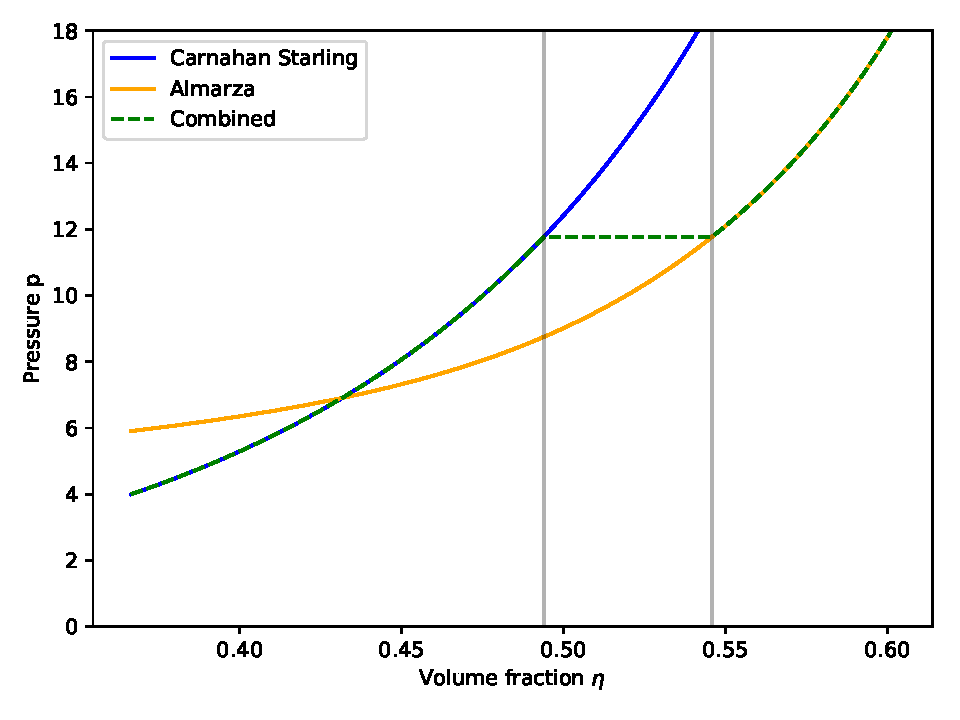
\includegraphics[width=0.7 \linewidth]{Hard_sphere_phase_diagram.pdf}
\caption[Phase diagram of hard sphere fluid]{Phase diagram of the hard sphere system with freezing and melting volume fraction shown as shaded lines and the green dashed line indicating the equilibrium stable branch. Where liquid and solid branch do not coincide with the stable branch, systems are unstable and tend towards a state on the stable branch.}
\label{fig:hs_phase_diagram}
\end{figure}
The equilibration solid fraction of the system $x_s = \frac{V_s}{V}$ with $V_s$ the solid volume and $V$ the total volume can be described by \autoref{eqn:solid_fraction_result}.\\ 
For the derivation it is necessary to use that in the stationary coexistence state the density of the solid phase is given by the melting density and that the liquid density is equal to the freezing density, i.e $\rho_s = \rho_{\text{melt}}$ and $\rho_l = \rho_{\text{freeze}}$ respectively. When further using the trivial equations
\begin{align}
V &= V_s + V_l \; \text{,} \nonumber\\
N &= n_s + n_l \; \text{,} \nonumber\\
N_i &= \rho_i V_i \; \text{,} 
\end{align}
with $n_{\text{s/l}}$ the number of solid/liquid particles we may write
\begin{align}
\rho V &= \rho_s V_s + \rho_l V_l \; \text{.}
\end{align}
This leads under the assumption of equilibrium within a few lines of calculation to 
\begin{align}
\frac{V_s}{V} &= \frac{\rho - \rho_{\text{freeze}}}{\rho_{\text{melt}} - \rho_{\text{freeze}} } \; \text{.}
\end{align}
As the solid fraction below $\rho_{\text{freeze}} $ vanishes and above $\rho_{\text{melt}}$ is 1, we can conclude that the equilibrium solid fraction of the system is given by \autoref{eqn:solid_fraction_result}.
\begin{align}
\label{eqn:solid_fraction_result}
x_s(\rho) = 
\begin{cases}
0 & \rho <  \rho_{\text{freeze}}\\
\frac{\rho-\rho_{\text{freeze}}}{\rho_{\text{melt}}-\rho_{\text{freeze}}} &  \rho_{\text{freeze}} < \rho <  \rho_{\text{melt}}\\ 
1 &  \rho > \rho_{\text{melt}} \quad \quad \text{.}
\end{cases}
\end{align}

Evaluating the above result at volume fractions where nucleations are accessible in simulations, between $\eta \in [0.53,0.55]$, leads to coexistence fractions of $x_s \in [0.7,1]$. This means that we are expecting nucleated systems to consist mostly of the solid phase after enough time for complete crystallization.\\

As pointed out earlier the phase transition takes place as it reduces the pressure in the liquid. This means that already during the growth of clusters the volume fraction of the metastable liquid is reduced, potentially altering its behavior significantly. For closer inspection of this the particle density of the metastable liquid depending on the solid fraction $x_s$ is evaluated in \autoref{eqn:meta_stable_volume_fraction}. For this purpose first the liquid volume $V_l$ and the number of liquid particles $N_l$ are expressed in terms of the solid fraction $x_s$:
\begin{align}
\label{eqn:volume_relation}
V_l(x_s) & = V(1-x_s)\\
\label{eqn:number_relation}
N_l(x_s) & = N-n_s(x_s) = N - \rho_m V x_s = N(1-\frac{\rho_m}{\rho}x_s)
\end{align}
Combining \autoref{eqn:volume_relation} and \autoref{eqn:number_relation} to the expression for the particle density in the remaining liquid leads to
\begin{align}
\label{eqn:meta_stable_volume_fraction}
\rho_l(x_s) &= \frac{N_l (x_s) }{ V_l(x_s) } = \frac{N}{V} \frac{1-\frac{\rho_m}{\rho}x_s}{1-x_s} = \rho \frac{1-\frac{\rho_m}{\rho}x_s}{1-x_s} \; \text{.}
\end{align}
%Some examples of \autoref{eqn:meta_stable_volume_fraction} are depicted in \autoref{fig:remaining_density} for moderate solid fractions of the system at regular volume fractions used for nucleation.\\
%\begin{figure}[h]
%\centering
%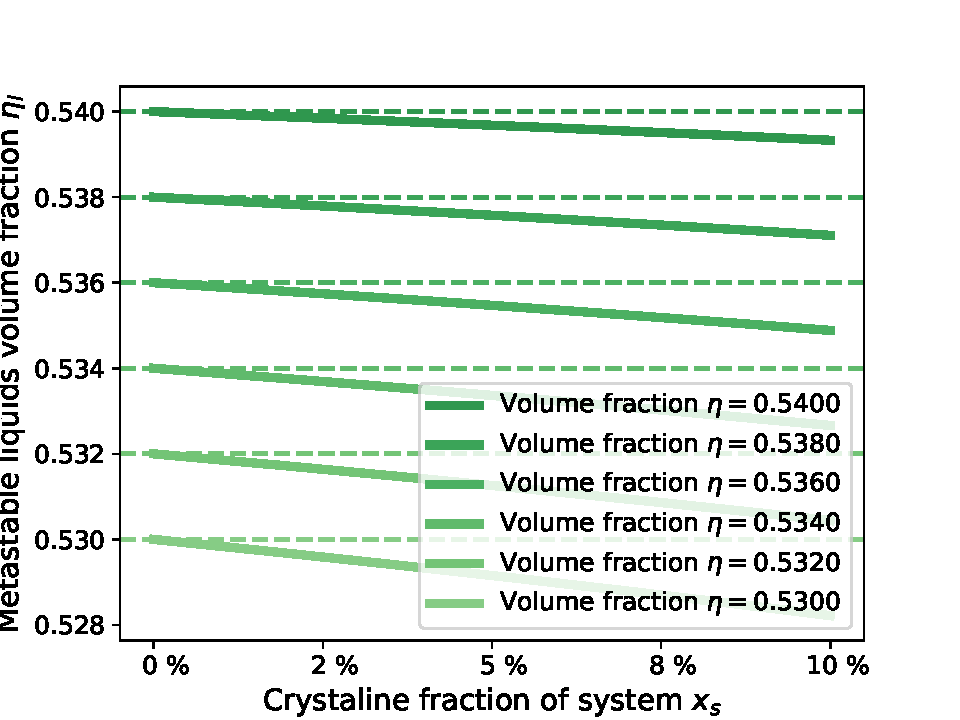
\includegraphics[width=0.5 \linewidth]{remaining_density.pdf}
%\caption[Density decrease of the fluid during crystallization]{Visualization of \autoref{eqn:meta_stable_volume_fraction}. The volume fraction of the remaining liquid decreases for all shown initial volume fractions only little up to crystalline ratios of a few percent.}
%\label{fig:remaining_density}
%\end{figure}
%What can be seen is that for crystalline fractions of a few percent the remaining liquid is not altered significantly. 
Evaluating the expression for relevant volume fractions of $\eta \in [53\%, 55\%]$ leads to the conclusion that crystalline fractions of $x_s < 5\%$ only reduce the packing fraction in the fluid by 0.1\%. Especially for system sizes of about 1 million particles this already corresponds to cluster sizes of a few ten thousand particles, where stable growth of clusters takes place which is rather insensitive to changes of the volume fraction as shown in \autoref{sec:cluster_growth}. This means that during the highly sensitive cluster forming processes the volume fraction of the liquid can be assumed to be globally stable.\\ 

%Eventhough not further discussed in this thesis it might be said that for polydisperse radii the phase diagram becomes even richer as show for example in 
%\todo{https://journals.aps.org/prl/pdf/10.1103/PhysRevLett.91.068301}

\section{Classical nucleation theory }
\label{sec:CNT}
Classical nucleation theory (CNT) has been proposed by Becker and Döring in 1935\cite{Becker1935} and since then used and modified multiple times to suit various types of systems. It still provides some reference or expectation, even if its framework does not seem to encompass the full nucleation process, to compare with the simulation data.\\

The simplest version of CNT assumes that a spherical crystallite of radius R may form in the liquid with properties of the bulk crystal while the fluid remains with the properties of the bulk fluid. The difference in the free energy landscape is given by a surface and a volume term, each depending on the radius. The first arises from the surface tension $\gamma$ between the fluid and the solid bulk phase, while the latter is caused by the difference in chemical potential $\Delta \mu$. The whole expression for the free energy is given by
\begin{equation}
\label{eqn:free_energy}
\beta \Delta G(R) =4 \pi R \gamma -\frac{4}{3} \pi R^3 \rho \Delta \mu  \; \text{,}
\end{equation}
with $\rho$ being the particle density of the solid phase.\\

For the difference of the chemical potential $\Delta \mu $ we first derive the free energy difference between the metastable liquid branch and the stable coexistence branch. To calculate the free energy we employ its differential relation
\begin{align}
\label{eqn:differential_relation}
dF = -S  \, dT -P \, dV + \mu  \, dN \; \text{.}
\end{align}
Setting the number of particles and the temperature constant and further reformulating $dV$ using \linebreak[1] $dN = dV  \, \rho + V  \, d\rho  $ and $dN = 0 $ we find $ dV = -d\rho \frac{N}{\rho^2}$. Under this transformation \autoref{eqn:differential_relation} becomes
\begin{align}
\label{eqn:df_relation}
\frac{dF}{N} = \frac{P(\rho)}{\rho^2} d\rho \; \text{.}
\end{align}

The pressure $P(\rho)$ is approximated by the Carnahan-Starling equation of state where we use $\eta = \frac{6 \rho }{\pi}$ and $Z=\frac{pV}{NkT} = \frac{p(\rho)}{\rho kT}$. Integrating \autoref{eqn:df_relation} between two densities $\rho_{1/2}$ hence is given by
\begin{equation}
\frac{\Delta F}{N} = \int_{\rho_1}^{\rho^2} \frac{kT}{\rho} \frac{1+\left( \frac{6 \rho}{\pi}\right) +\left( \frac{6 \rho}{\pi}\right)^2 - \left( \frac{6 \rho}{\pi}\right)^3}{\left( 1 - \frac{6 \rho}{\pi}\right)^3} d\rho \; \text{,}
\end{equation}
with the analytical solution
\begin{equation}
\int_{x_1}^{x_2} \frac{1+(ax) +(ax)^2 - (ax)^3 }{( 1 - ax )^3 \,  x} dx = \left. \frac{3-2ax}{(ax-1)^2} + \text{log}(x) \right|_{x=x_1}^{x_2} \; \text{.}
\end{equation}
Dropping the lengthy notation for $\eta$ we end up with
\begin{equation}
\frac{\Delta F}{N} = kT \left(  \frac{3-2 \eta_2}{(\eta_2 - 1)^2} - \frac{3-2 \eta_1}{(\eta_1 - 1)^2} + \text{log}\left( \frac{\eta_2}{\eta_1} \right) \right) \; \text{.}
\end{equation}
The analytical solution is compared in \autoref{fig:free_energy_diff} with numerically results which have been calculated before the analytical solution was found. In the following the free energy difference is identified with the difference in chemical potential $\Delta \mu$ as it is the driving force of the nucleation.\\
\begin{figure}[h]
\centering
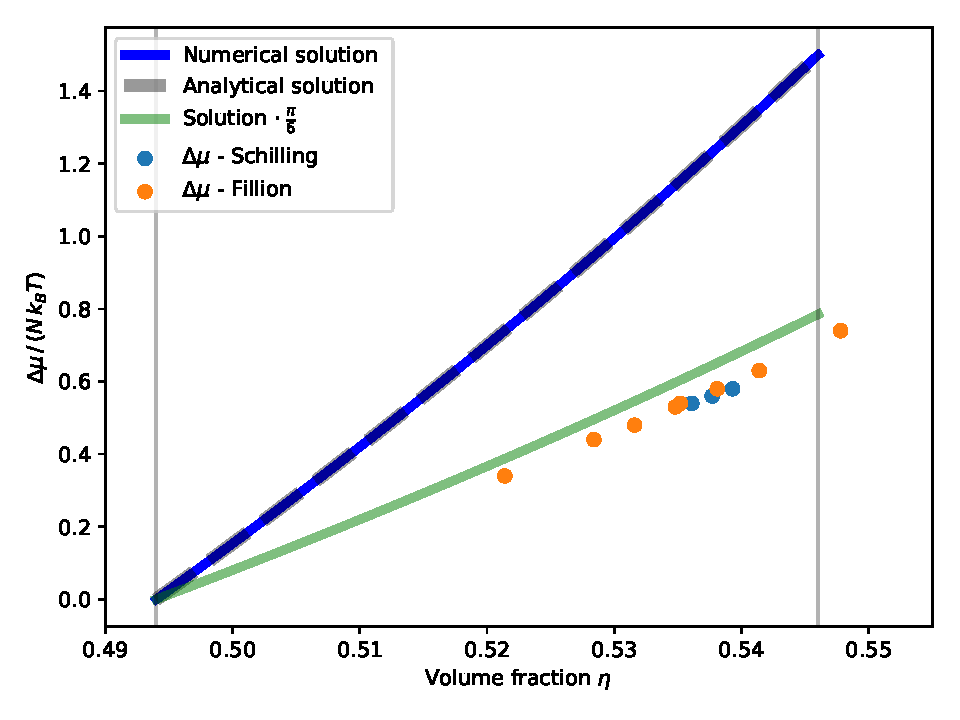
\includegraphics[width=0.7 \linewidth]{Free_energy_difference.pdf}
\caption[Free energy difference between fluid and solid phase]{Free energy difference per particle between the metastable liquid phase and the coexistence phase. Values by Schilling et al. 2011\cite{Schilling2011} and Filion et al. 2010\cite{Filion2010a} deviate from the shown result, but we assume that a factor of $\frac{\pi}{6}$ in the calculations is missing in either this or their calculation, as the modified green curve collapses rather accurately on the literature values when choosing $\eta_{\text{freeze}}=0.5$.}
\label{fig:free_energy_diff}
\end{figure}


Coming back to the free energy landscape of \autoref{eqn:free_energy}, we see that it exhibits a maximum at a radius called $R_{\text{crit.}}$. The interpretation of this radius is that if a cluster surpasses the critical radius it is likely to keep growing until the system settles at the equilibrium solid fraction. Here a cluster is defined as a structure having a locally crystalline like ordering. The critical radius, simply calculated by setting the derivative of \autoref{eqn:free_energy} to zero, is given by
\begin{equation}
\label{eqn:r_crit}
R_{\text{crit.}} = \frac{2 \gamma}{\rho \Delta \mu } \; \text{,}
\end{equation}
and the height of the barrier at the critical radius is given by
\begin{equation}
\beta \Delta G (R_{\text{crit.}}) = \frac{16 \pi \gamma^3}{3 \rho^2 (\Delta \mu )^2} \; \text{.}
\end{equation}

The classical critical radius depending on the volume fraction is depicted in \autoref{fig:r_crit} for a first impression of the cluster sizes that we are expecting for nucleation. The interfacial surface tension for this often is given by $\gamma \approx \SI{0.6}{k_B T \sigma^{-2}}$, but its precise value is under debate. Thus we may stick to one of the recently calculated values of $\gamma = \SI{0.589}{k_B T \sigma^{-2}}$ by Bültmann and Schilling 2020\cite{Bultmann2020}. 
\begin{figure}[h]
\centering
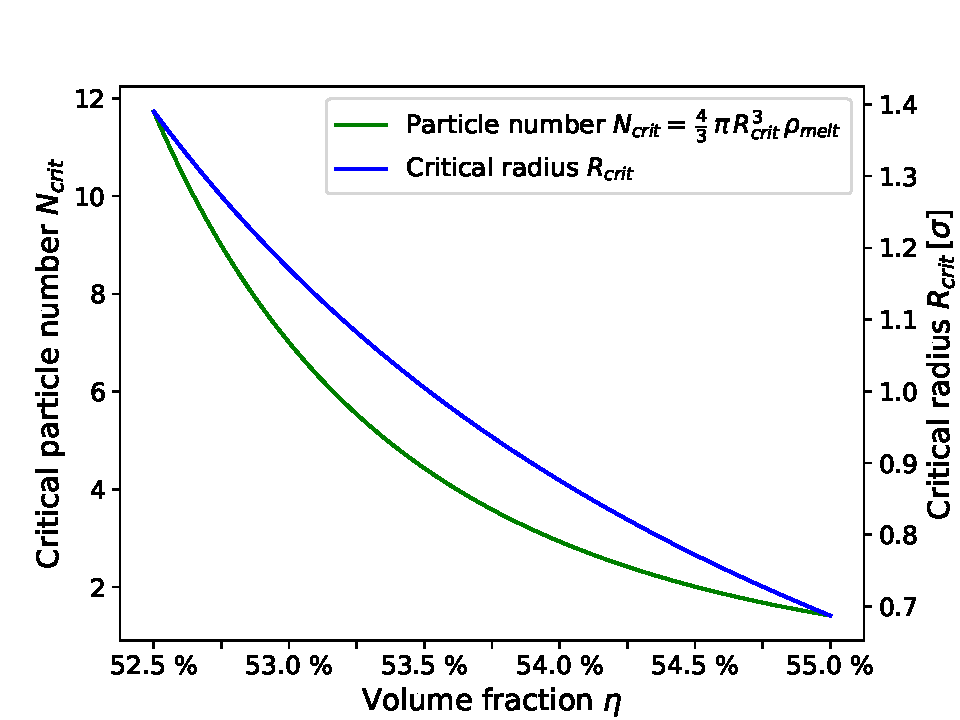
\includegraphics[width=0.7 \linewidth]{CNT_radius.pdf}
\caption[Critical radius in the metastable regime]{Critical radius $R_{\text{crit.}}$ calculated from CNT depending on volume fraction $\eta$. The critical radius obtained by our calculation is rather small, but when using the chemical potential calculated by Schilling and Filion the critical cluster size is of the order $N \approx 50$ at intermediate metastable volume fractions, corresponding better to typical fluctuations of the largest cluster found in simulations.}
\label{fig:r_crit}
\end{figure}

\section{Computer precision and chaotic behavior}
\label{sec:precision}
The finite floating point precision impacts the outcome of the simulation as it constitutes a many body problem with chaotic behavior. In this section it is shown that even smallest variations of positions for example, lead to radical changes of the simulation after a certain number of steps. It is used to emphasize the importance to rigorously save the simulation state if it is supposed to be restarted from file, or with changing measurement intervals. Also it reminds us that the numerical simulation only is an approximation that never follows the phase space trajectories of the true system.\\

The exponential growth of induced variations in a chaotic system can be visualized by comparing a reference simulation with a perturbed one. In \autoref{fig:chaotic_behavior} the mean of the squared displacements of all particles is recorded between such a pair of simulations. The perturbation consists of a slight push of $10^{-10} \sigma$ to one particle's position, comparable with missing some floating point precision during saving and loading.\\

\begin{figure}[h]
\centering
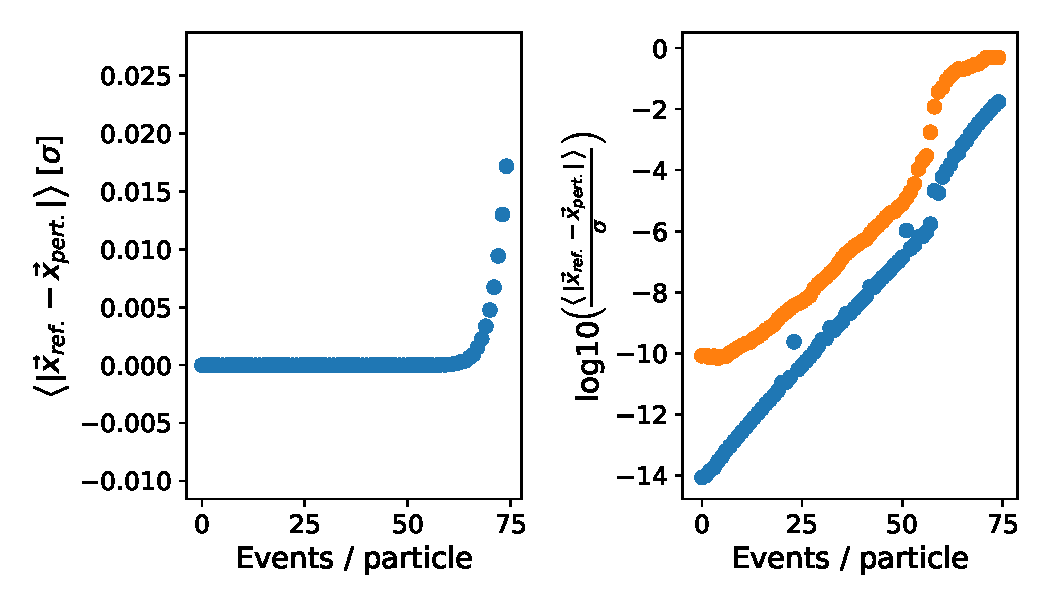
\includegraphics[width=0.7 \linewidth]{perturbation.pdf}
\caption[Exponential growth of perturbations in chaotic system]{Mean difference of particle positions in the reference and perturbed simulation. The blue lines show the same data while the orange curve shows the maximum deviation present at each step. For comparison with datasets using the system time $\delta t$ as units, a rough conversion is given by $T \approx \text{(\#steps)} \cdot \frac{1 \delta t}{60 \text{steps}}$, where a step is defined as one event execution per particle.\\ The maximum deviation first consists only of the initial perturbation but then increases similar to the mean deviation.}
\label{fig:chaotic_behavior}
\end{figure}

While only observing the left side leads to the assumption that the simulations remain the same to a certain point and then suddenly diverge, in the logarithmic representation we see that actually the perturbation grows exponentially as long as it is small and deviates from this exponential growth at some point when reference and perturbed simulation become more or less independent of each other.\\
The small bumps at first sight seemed to be an artifact of the periodic boundary conditions but this seems not to be the case. What causes these deviations therefore remained hidden.\\

The challenge that this behavior poses is that any perturbation pushes the system to a completely different trajectory. In the context of EDMD simulations we can for example look at the case when a measurement of some quantity is performed. For this purpose all particles have to be propagated to the global time. To not perturb the system with this extra calculations, an exact copy of the particle positions has to be saved prior to the measurement. Following it, this copy is then used to restore the unperturbed system.\\ 
Similarly recalculating an event for the FEL at some point of time is not possible as the outcome will vary in the last digits. For this reason it becomes necessary to save all precalculated events of the simulation to be able to restart it from a file.\\
But facing this challenge makes it possible for example to resimulate an interesting part of a trajectory from some saved checkpoint with a higher measurement frequency to resolve more details. 

\section{Comparison to real world experiments} 
\label{sec:comparison}

Starting in 1986 with the experiments by Pusey and Megen\cite{Pusey1986}, hard sphere like systems have been synthesized in the laboratory. Today a large variety of such is known, but still further systems are developed to better control stability, sphere size or also to reduce the possible impact of charges on top of the spheres as the Coulomb interaction alters the behavior of the system. Still all of these systems have in common that the hard spheres are suspended in some fluid. Even though nucleation experiments can be done without gravity in space\cite{Doherty1998}, usually the fluid's mass density has to be matched to the mass density of the hard spheres to prevent sedimentation. Further it is necessary for optical measurements to match the refractive index of the fluid and the spheres as otherwise the probe becomes opaque .\\

The absence of the bath in simple hard sphere simulations constitutes a large difference to those experiments in the laboratory. It has been argued that this only introduces a difference of the time scale which can be compensated by using the characteristic diffusion time as the unit of time, but a discussion on the possibility of hydrodynamic effects changing the behavior of the laboratory system compared to simulations is ongoing at the moment, see Radu and Schilling 2014\cite{Radu2014} compared to Fiorucci et al. 2020\cite{Fiorucci2020a}.\\
Also the mode spectrum of the suspending fluid within the cavities between the dispersed spheres might have a more important role 
than expected, but requires further investigation.\\ 
Still it usually is not possible to include the suspending fluid into simulations as the proliferation of particles raises calculation times by orders of magnitude.\\

A further difference is given by the spatial extent and geometry of the simulation. The geometry in simulations is often defined by periodic boundary conditions (PBC) to circumvent surface effects, which is a rather unphysical setup.\\ 
Concerning the spatial extent, simulations are mostly confined to very small systems in comparison to experimental setups leading to a further major difference between the measurement geometries: While the experimentalists usually probe a continuous volume of hard spheres in a suspending fluid, in simulations many disjunct volumes are used as each subvolume can be processed by one CPU, making simple parallelization of the calculations possible. While the expected behavior of disjunct volumes under the assumption of a constant nucleation rate is discussed in \autoref{sec:induction_time_expectation},












 the overall solid fraction of a volume in the thermodynamic limit is inspected in the following.\\

In \autoref{sec:cluster_growth} the cluster growth rate $c$ is found to be mostly independent of the volume fraction in simulations. When extrapolating from the small region in which it was tested, we may approximate the number of particles $N$ at time $t$ for a cluster that emerged at time $t_0$ by
\begin{align}
\label{eqn:simple_growth}
N(t) = c^3 (t-t_0)^3 \; \text{.}
\end{align} 
Furthermore approximating the stochastic nucleation events with rate density $\kappa$ by instead just adding a new cluster after every $\Delta t = (\kappa V)^{-1}$, we can write the total number of solidified particles $N$ in a Volume $V$ at time step $m$ with the corresponding time $t_m = m \Delta t$ as the sum of all previously nucleated cluster sizes $N_i$. Reformulating this leads to
\begin{align}
\begin{split}
N(t_m)&=\sum_{i=1}^m N_i\\
\Leftrightarrow N(t_m)&=\sum_{i=1}^m N_i \frac{\Delta t}{\Delta t}\\
\Leftrightarrow N(t_m)&=\kappa V \sum_{i=1}^m N_i \Delta t\\
\Leftrightarrow N(t_m)&=\kappa V \sum_{i=1}^m c^3 (t_m-t_i)^3 \Delta t
\end{split}
\begin{split}
\label{eqn:x_s_t_lim}
\stackrel{V \rightarrow \infty } {\Leftrightarrow} \quad N(t)&=\kappa V \int_0^{t} c^3 (t - t')^3 d t'\\
\Leftrightarrow \; \, \frac{N(t)}{V \rho_{\text{melt}}}&=\frac{\kappa c^3}{\rho_{\text{melt}}} \left. \frac{1}{4}t''^4 \right|_{t''=0}^t\\
\Leftrightarrow \; \; \; \; \frac{V_{solid}}{V} &= t^4 \frac{\kappa c^3}{4 \rho_{\text{melt}}}\\
\Leftrightarrow \quad \; \: x_s(t)&= t^4 \frac{\kappa c^3}{4 \rho_{\text{melt}}}
\end{split}
\end{align}
Here the solid fraction is not the equilibrium solid fraction, but rather the expected solid fraction of an infinitely large system at a time $t$ after some quench that suddenly takes the system into the metastable regime.\\ 
For the derivation of \autoref{eqn:x_s_t_lim} the thermodynamic limit $V\rightarrow \infty$ is used to obtain the definition of an integral. Further it neglects any interference between different clusters. This assumption is justified for $x_s \ll 1$ if no long range interference is present and heterogeneous nucleation is assumed to be part of the cluster growth process.\\

With this we can calculate a characteristic nucleation time $t^*$ at which $x_s$ is not negligible anymore. As in simulations with periodic boundary conditions clusters begin to interfere with each other at a filling fraction of about $x_s=\frac{1}{8}$, which is also chosen as a threshold where interference can not be neglect any longer in the macroscopic system. Under this definition $t^*$ becomes
\begin{align}
\label{eqn:nucleation_time_modified}
t^* = \sqrt[4]{\frac{\rho_{\text{melt}}}{2 \kappa c^3 }} \; \text{.}
\end{align}
As we see the time $t^*$ actually depends only on the fourth root of the induction time $\tau_{\text{nucleation}} = \kappa^{-1}$. This might be an explanation for the huge discrepancy between experiment and simulation studies, as can be seen in \autoref{fig:nucleation_rate_comparison_modified}, where the inverse of $t^*$ is calculated from different simulation studies and depicted together with experimentally found nucleation rates.\\
\begin{figure}[h]
\centering
%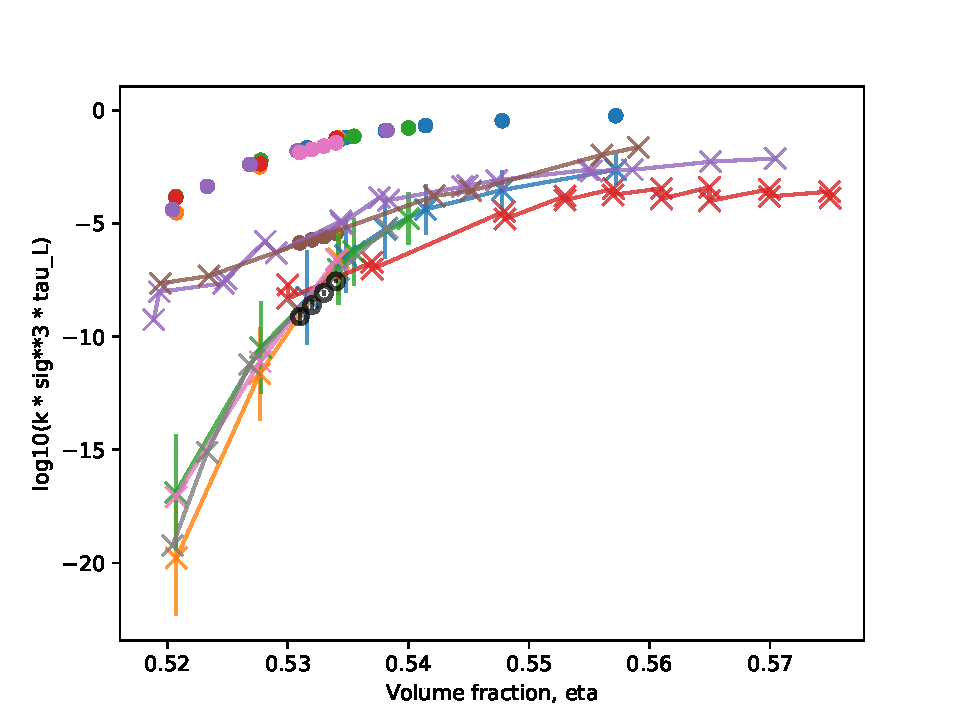
\includegraphics[width=0.6 \linewidth]{t_fill_rate_comparison.pdf}
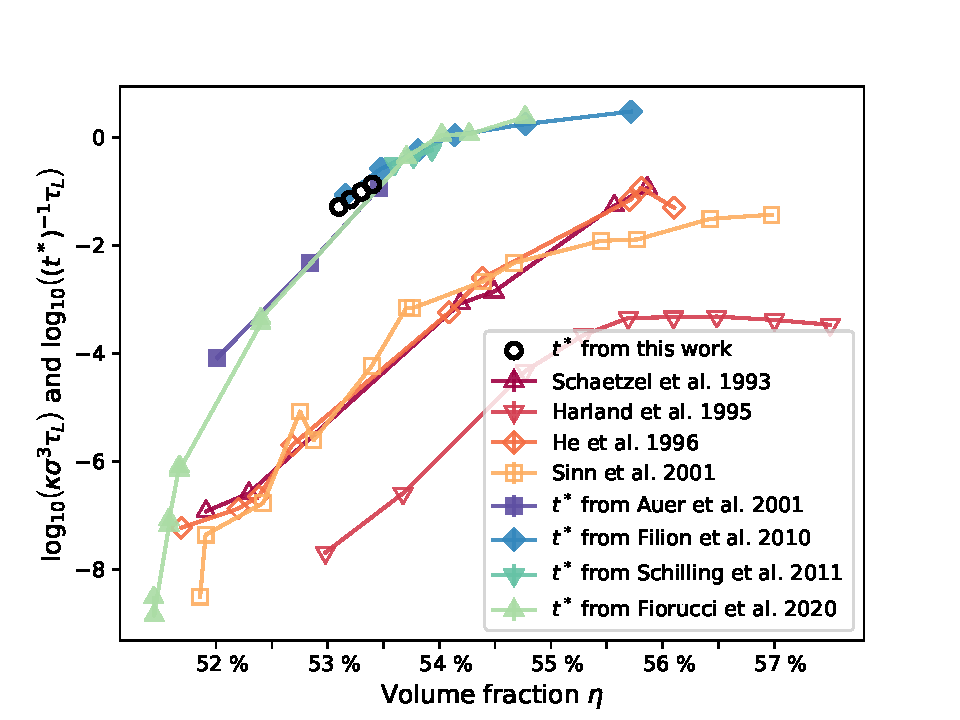
\includegraphics[width=0.7 \linewidth]{mod_nucleation_comparison_v2.pdf}
\caption[Nucleation rate comparison under assumption of early filled boxes]{Diagram with experimentally measured nucleation rates\cite{Harland1997,He1996,schaetzel1993,Sinn2001,Auer2001} as well as $(t^*)^{-1}$ calculated from nucleation rates obtained in simulation studies\cite{Filion2010a,Fiorucci2020a,Schilling2011}. The set of datapoints is equivalent to those of \autoref{fig:nucleation_comparison}.}
\label{fig:nucleation_rate_comparison_modified}
\end{figure}

What can be seen is that the gradient of $(t^*)^{-1}$, calculated from the simulation results, follows mostly the one of the experimental results as the fourth root changes the slope by a factor of 4 in the logarithmic diagram. The rates still deviate by a factor of about 10000 which still requires explanation.\\

While this is not a proof it might be a hint that laboratory based experiments measure more cluster growth than actual nucleation events. It has to be discussed with experimentalists if the assumptions leading to this result hold under closer inspection or if measures against this behavior have been taken.

\newpage

\chapter{Simulation details}
% !TEX root = writing_version.tex

\label{chp:simulation}
During the coarse of the master thesis an event driven molecular dynamic (EDMD) simulation code has been elaborated. The choice to use the EDMD approach is taken because interst in the actual dynamics of the system were desired. This means that simulations probing the phase space of the system instead of the dynamics, like Monte Carlo (MC) simulation schemes, are not suited.\\ 
Furthermore the discontinous potential of the hard spheres is an obstacle not easy to face in regular molecular dynamics (MD) schemes, where the Newtonian equation of motion for the particles is numerically integrated.\\
The EDMD approach on the other site actually requires these discontinuities as will be discussed in the following sections, together with some details of the program.\\

\section{Algorithm and Simulation details}
\label{sec:simulation}
%EDMD and Simulation details
In this section we will highlight the main differences to regular MD simulations, as they are the main tool to otherwise probe the dynamics of the system. Furthermore we will stick to the hard sphere example when discussing the EDMD simulations, but it can be kept in mind that the EDMD approach also allows to simulate particles with other potentials as long as the potentials are only containing step functions.\\
 
The decisive difference between EDMD simulations and regular MD schemesis that, instead of evaluating all pair and external forces on each particle and then evolving the whole system to the next time step, EDMD simulations do not have a predefined time step, but the system is evolved from one event to the next one. An event in this context is defined as the time where the next collision in the whole system takes place.\\

The event prediction algorithm is follows closely the approach proposed by Bannerman et. al \cite{Bannerman2014} which will be discussed in the next section.\\

\subsection{Event driven molecular dynamics (EDMD)}
\label{sec:EDMD}
For the prediction of events in EDMD simulations an overlap function $f_{ij}(t)$ between particles i and j is defined, where the squared quantities are used merely because they are easily accessible.\\
\begin{align}
f_{ij}(t) & \coloneqq  | \vec{r}_j(t) - \vec{r}_i(t) |^2 - \sigma^2\\
          & \; \; \, \vrule
  \begin{aligned}[t]
    \quad \text{with} \quad \vec{r}_i(t) &= \vec{r}_i(t_0) + (t-t_0) \; \vec{v}_i(t_0) \, \text{,}\\
    \Delta t \coloneqq & \; t-t_0  \, \text{,} \\ 
    \vec{v}_{ij}(t) &\coloneqq  \vec{v}_j(t) - \vec{v}_i(t) \, \text{,}\\
    \vec{r}_{ij}(t) &\coloneqq  \vec{r}_j(t) - \vec{r}_i(t) \, \text{,}\\
    \Leftrightarrow \quad \vec{r}_{ij}(t) &= \vec{r}_{ij}(t_0) + \Delta t \; \vec{v}_{ij}(t_0)
  \end{aligned}\\
f(t)  & = ( \vec{r}_{ij}(t_0) +  \Delta t \;  \vec{v}_{ij}(t_0))^2 -\sigma^2 \\
\label{eqn:overlap_f}
f(t)  & = |\vec{r}_{ij}(t_0)|^2 + \Delta t ^2 \; |\vec{v}_{ij}(t_0)|^2 - 2 \Delta t \; \vec{r}_{ij}(t_0) \cdot \vec{v}_{ij}(t_0)  -\sigma^2
\end{align}  

The overlap function has the property that it is negative for two particles being closer than their diameter, 0 for at collision and positive if neither overlapping nor touching. The calculation of the next collison thus is to calculate the roots of \autoref{eqn:overlap_f}.\\

%Solving it \todo{go to the library and take again the book to write from it the solution}
Solving for $\Delta t$ with $|\vec{r}_{ij}(t_0)|^2 \coloneqq rr $, $|\vec{v}_{ij}(t_0)|^2 \coloneqq vv $ and  $\vec{r}_{ij}(t_0) \cdot \vec{v}_{ij}(t_0) \coloneqq rv $ is rather trivial:
\begin{align}
0 &= rr + vv \; \Delta t ^2  - 2 rv \; \Delta t  -\sigma^2\\
\Leftrightarrow \quad 0 &= \Delta t ^2 - \frac{2rv}{vv} \; \Delta t + \frac{rr - \sigma^2 }{vv}\\
\Leftrightarrow \, \, \Delta t &= - \frac{rv}{vv} \pm \sqrt{\left(\frac{rv}{vv}\right)^2 - \frac{rr - \sigma^2 }{vv}}
%\label{eqn:collision_prediction_pre}
%\Leftrightarrow \, \, \Delta t &= \frac{ - rv \pm \sqrt{ (rv)^2  - vv (rr - \sigma^2 )} }{vv}\\
%\Leftrightarrow \, \, \Delta t &= \frac{rv \pm \sqrt{ (rv)^2  - vv (rr - \sigma^2 )} }{vv} \; \frac{ - rv \mp \sqrt{ (rv)^2  - vv (rr - \sigma^2 )}}{ - rv \mp \sqrt{ (rv)^2  - vv (rr - \sigma^2 )}}\\
%\label{eqn:collision_prediction}
%\Leftrightarrow \, \, \Delta t &= \frac{(rr - \sigma^2 )}{ - rv \mp \sqrt{ (rv)^2  - vv (rr - \sigma^2 )}}
\end{align}
%To circumvent a caveat when executing on a floating point machine, \autoref{eqn:collision_prediction_pre} is rewritten as in \autoref{eqn:collision_prediction}.\\ 

But a caveat when executing on a floating point machine is present as can be seen when considering which solution is of interest. As for a possible collision it is necessary that the two particles move towards each other we can conclude that the scalar product is required to be negative $rv<0$, because otherwise the particles are already moving away from each other.\\ 

Also the quadratic formula has two solutions, corresponding to the entry and the exit of the overlap. Because the entry has to be prior to the exit, we further conclude that interest lies on the smaller solution that is:
\begin{align}
\label{eqn:collision_prediction_pre}
\Delta t &= \frac{ - rv - \sqrt{ (rv)^2  - vv (rr - \sigma^2 )} }{vv}
\end{align}
Now for the case where the distance of the spheres is already close to the diameter of the spheres we find $(rv)^2 \gg (rr-\sigma^2)$, which results in a cancelation of two large numbers leaving a small number. Floating point number operations are inherently bad suited because they tend to large inaccuracy in this case. Rewriting \autoref{eqn:collision_prediction_pre} by making use of the third binomial formula \todo{look if this is fine to write.} leads to:
\begin{align}
\label{eqn:collision_prediction}
\Delta t &= \frac{(rr - \sigma^2 )}{ - rv + \sqrt{ (rv)^2  - vv (rr - \sigma^2 )}}
\end{align}
Comparably \autoref{eqn:collision_prediction} does not contain a cancelation of the type seen before and such is better suited for the use in a computer simulation. \todo{cite Goldberg '91}\\

%The algorithm proposed by Bannermann\cite{Bannerman2014} works by differentiating 4 cases:
%\begin{description}
%\item[First,] \hfill \\ if $rv>0$ the particles move away from each other leading to a collision time of $\Delta t = \infty$.
%\item[Second,]\hfill \\ if $rr<\sigma^2$ an overlapis present resulting in an immediate collision time of $\Delta t = 0$
%\item[Third,] \hfill \\ if $(rv)^2  - vv (rr - \sigma^2 ) \leq 0 $ the two particles miss each other, including touching without momentum transfer, resulting in a collision time of $\Delta t = \infty$
%\item[Fourth,] \hfill \\ if none of the before is given the particles collide and $\Delta t$ is calculated by \autoref{eqn:collision_prediction}.
%\end{description}

The event prediction algorithm proposed by Bannermann\cite{Bannerman2014} works by differentiating 4 cases:
\begin{enumerate}
\item If $rv>0$ the particles move away from each other leading to a collision time of $\Delta t = \infty$.
\item If $rr<\sigma^2$ an overlap is present resulting in an immediate collision time of $\Delta t = 0$
\item If $(rv)^2  - vv (rr - \sigma^2 ) \leq 0 $ the two particles miss each other, including touching without momentum transfer, resulting in a collision time of $\Delta t = \infty$
\item If none of the before is given the particles collide and $\Delta t$ is calculated by \autoref{eqn:collision_prediction}.
\end{enumerate}

All collision times for a particle are then stored in a queue sorted by event time called particle event list (PEL). From the PEL the first entry is then passed to the global FEL.\\
This procedure initally takes place for all particles to set up the system and later on for particles involved in an event after its execution.\\ 

As will be discussed in \autoref{sec:implemetation} some redundant calculations have been omitted in the actual simulation program, as well as a cell system added to reach $\mathcal{O}(N)$ computation time, in turn introducing a new event type for cell changes.\\

A further detail to take care of is the possibility of scheduled events which have bcome invalid due to a earlier collision of the one of the particles. This is handeled by assigning an interaction count to each particle and then store this at precalculation time with the event. When the event comes up, and the interaction count of one of the particles has increased in the meantime, the event is said to be invalidated. Depending on which particle had an event in the meantime the invalidation either causes no action or a recalculation of new events.\\  

\subsection{Details of the Implementation} 
\label{sec:implemetation}
%Add Details of for example FEL, and backupevent handling, double time precision, reset sim
As the simulation code is based on an earlier Monte Carlo Code for hard spheres a complete walk through the whole progam would become quite extensive. Such we will focus on key points to understand the details of the simulation.\\

\subsubsection{\textit{Event} struct}
\label{sec:event_struct}
We start with the basic \textit{Event} struct which includes 6 entries as shown in \autoref{tab:event_entries}.
\begin{table}[h!]
\centering
\begin{tabular}{c|c}
\textbf{Datatype} & \textbf{Name of entry}\\ \hline
(timeType) & time \\
(int) & event\_type \\
(particle*)  & particle \\
(void*) & partner \\
(int) & particle\_count \\
(int) & partner\_count \\
\end{tabular}
\caption{Content of the \textit{Event} struct.}
\label{tab:event_entries}
\end{table}
The type of \textit{time} (timeType) is usually set to double. The \textit{time} variable itself represents the time for when the event is scheduled.\\ 
The \textit{event\_type} variable is either set to 0 or 1 and indicates if the event is a cell transfer or a collision of two particles.\\
The \textit{particle} variable is a pointer to the particle for which the event has been pre calculated, while the \textit{partner} variable is set to be a void pointer. Such it is possible to either interpret it as a particle pointer for the collision type event or as an interger pointer to the index in the current cells' neighbours list for transfer events.\\
In the last two rows the interaction counts for particle and partner are listed as well. As the destination cell in a transfer event does not require an interaction count, the \textit{partner\_count} variable is only used for collision events.\\

The \textit{event} struct is used for all events throughout the simulation. For read and write operations with the HDF5 file format, the struct \textit{event\_data} is available which uses only indexes instead of pointers.\\

\subsubsection{\textit{Particle} class}
\label{sec:particle_class}
The \textit{Particle} class is comparably to the one from the MC code basis. Its MC related variables have been removed and additional key variables and concepts will be discussed in the following:\\

First a vector storing events called \textit{backupEvent} has been added to make it possible to store events from the pre calculation for the case of the first event being invalidated. The idea of reusing events is discussed in many publications, for example that the memory cost increases onyl moderately with more backup events while the speedup does not increase much for more than two stored events \cite{Bannerman2011}. It also has been argued that the added complexity can not account for the increase in efficency\cite{DONEV2005}.\\ 
Eventhough in the own simulations a decrease in calculation time of more than 10\% was observed and the cost of complexity was seen as moderate. The difference might be explained by the fact that the systems under consideration in this thesis have a rather large particle density, leading to more invalid collsions.\\

In the context of reusing pre calculated results, it should also be mentioned that after a cell transfer the recalculation of events can be restricted to partner particles only in the new neighbouring cells, leading to only 1/3 of the calculation time in this case. But as mentioned systems under consideration are mostly rather dense and such the number of transfers is often at below 5\%. Thus the increase in efficency was assumed to be to costly on the complexity side, and not implemented. Eventhough for sparse systems, it might make sense to include an \textit{updatePEl} routine.\\


Also key differences to the former MC Particle type are the variables \textit{total\_interactions} and \textit{particle\_delayed\_time}. The first is the variable for book keeping of interactions, while the second represents the event driven character of the simulation. Because each particle only moves on purely ballistic trajectories until an event occurs, it is not necessary to keep all particle positions and velocities synchronized in time. Quite on the contrary it would mean executing extra operations together with summing rounding errors by each floating point operation.\\

Because sometimes it is desired to have the whole configuration at one point of time, the \textit{transferToTime()} function of the particle provides the possibility to take the particle into the present. This is necessary soon as measurements are performed on the system, including snapshots.\\

As mentioned before the system behaves chaotic even under slightest changes like a rounding error from an extra floating point operation. A result of this is that measuring at different rates during a simulation changes the simulation trajectory quite a bit. It has been observed that such a system may keep close to the undisturbed trajectory for about 50-100 events/particle. As it is of desire to measure quantities and take snapshots without disturbing the simulation, the simulation program makes employs copies of the configuration being costly in terms of memory but making simulation resets or higher sampling rates at interesting points possible within a defined trajectory.\\ 

The structure is as follows: The first copy is rewritten with an image of the working configuration just before any measurement. The working trajectory iteself is then disturbed by the measurement, and afterwards replaced with its state before the measurement from the backup configuration.\\
The second copy actually includes the full simulation state, while the first only includes the particle cofiguration. This second one might be used to save a state during the simulation and reset to just the same point at any later time.\\


\subsubsection{The \textit{Box} class}
\label{sec:box_class}
The box of the simulation stayed mostly the same as in the previous MC code. One chanege is the array \textit{neighbours\_lookup} which has been added. It contains the indices for the cells' \textit{neighbours} array pointing to cells that share their surface. It is used to identify which cell a particle has to be transfered to during a cell transfer event.\\

Furthermore the \textit{Update} routine now takes care of all quantities depening on the length of the box, making the \textit{rescale} routine a simple rescaling of the edge lengths with an additional \textit{Update} command.\\

\subsubsection{The \textit{Scheduler} class}
\label{sec:scheduler_class}
While the afore mentioned parts of the program are necessary for the EDMD program, the \textit{Scheduler} class contains the most distinct parts of the program. It keeps track of all events to come, predicts new events and orchestrates the execution of the events. The essential functions are discussed in the following subsections while some basic properties are shortly highlighted here.\\

First of all the \textit{Scheduler} holds the Future event list (FEL) in which at least one event per particle is stored. As discussed within \autoref{sec:particle_class} the simulation is capable of saving the complete state of a trajectory, including all pre calculated events. For this purpose an array of \textit{Events} is available.\\
Furthermore the \textit{Scheduler} includes the \textit{gloabl\_time}.\\
Important for the efficency is the pre allocation of all arrays used within the prediction calculations, as the number of executions for the collision prediction routine is about $\frac{30}{\text{particle} \cdot \text{step}}$ accounting to a few billion function calls during a small simulation.\\

\subsubsection{\quad \textit{Scheduler::predictTransfer()}}
As the name suggests this function predicts the next cell transfer of a particle due to its movement. For this it calculates the position of the particle at global time, which for a valid state of the simulation always lies within its cell. By transforming the momentary position of the particle from the global coordinate system to the coordinate system of the cell and taking into account the periodic boundary conditions, we can write for each dimension $i$ the equations
\begin{align}
t_{i1}=-\frac{r_i}{v_i} \quad \text{and} \quad t_{i2}=\frac{l_i-r_i}{v_i}
\end{align}
which describe the times when the particle pierces the cell's left and right boundaries. A negative time corresponds in this case to a boundary crossing in the past, a time comparable to 0 means that the particle is on the edge of its cell and a positive time means that the boundary crossing lies in the future. By going through the different possible cases for $t_1$ and $t_2$ we find the resulting next crossing time for each case as shown in \autoref{tab:crossing_times}.
\begin{table}[h]
\centering
\begin{tabular}{c|c||c|c}
$t_1$ & $t_2$ & Result & Case \\ \hline
> & > & invalid & - \\ \hline
> & = & $t_{\text{crossing}} = t_1$ & 0 \\ \hline
> & < & $t_{\text{crossing}} = t_1$ & 1 \\ \hline
= & > & $t_{\text{crossing}} = t_2$ & 2\\ \hline
= & = & invalid & - \\ \hline
= & < & $t_{\text{crossing}} = t_1$ & 3 \\ \hline
< & > & $t_{\text{crossing}} = t_2$ & 4 \\ \hline
< & = & $t_{\text{crossing}} = t_2$ & 5\\ \hline
< & < & invalid & - \\ \hline
\end{tabular}
\caption{Possible results for left and right crossing time with resulting choice of next crossing time. >, = and < are to be read as for example $t_1 > 0$. The case indicates the case number within the actual simulation.}
\label{tab:crossing_times}
\end{table}

By collecting the next crossing times for each dimension and taking the minimum of these times the exit time of the particle from its cell is determined.\\

The return value of the routine is an \textit{Event} where the partner is given as an address to the box' \textit{neighbours\_lookup}. The index lies between 0 and 5, corresponding to the 6 possible neigbhour cells sharing a surface with the current cell of the particle. Each valid case represents a distinct neigbour cell and the index within the cells \textit{neighbours} array is clearly defined by the cell setup routines and is shown in \autoref{tab:cell_neighbour_index}. 

\begin{table}[h]
\centering
\begin{tabular}{c|c|c|c}
dimension & boundary & case & index \\ \hline
x & front & 0 & 12 \\
 & back & 1 & 13 \\ \hline
y & front & 2 & 10 \\
 & back & 3 & 15 \\ \hline
z & front & 4 & 4 \\
 & back & 5 & 21 \\
\end{tabular}
\caption{Overview of the cells' \textit{neighbours} indices directly sharing a surface for 3 dimensions. As the indices hardly follow any simple pattern they are explicitly noted at this point. Obviously the cell consists of a front and a back boundary in each dimension. The corresponding case matches the one from \autoref{tab:crossing_times}.}
\label{tab:cell_neighbour_index}
\end{table}
\FloatBarrier

\subsubsection{\quad \textit{Scheduler::predictCollision()}}
The prediction of collision times has already been discussed in \autoref{sec:EDMD}. The implementation in the program first calculates all necessary scalar products while accounting for the periodic boundary conditions, and in a second step returns the collision time depending on the case at hand.\\

The presented algorithm is only valid for single sized particles. If polydisperse systems are supposed to be considered the algorithm has to be adjusted. \todo{mayhap do it in the appendix?}\\

As this routine is executed through out the simulation very often it has been tried to optimize its efficency multiple times. For example calculating only necessary results for the next case differentation has been implemented but no significant increase in efficency was recognized and for better readability the prior version has been reestablished. In either case if an optimized way of calculating the results is found it might be useful to use them.\todo{<-- Not really nice}\\    

\subsubsection{\quad \textit{Scheduler::setupFEL()}}
This routine fill the FEL of the simulation. For this purpose it iterates through all particles and calls \textit{setupPEL} for each of them. The PEL in turn is set up by predicting the next cell transfer as well as the next collisions with all particles within the $3^d$ cells directly surrounding the particle. From all predicted events only such with finite times are then written to the \textit{backupEvents} vector corresponding to the PEL of the particle.\\
For the FEL only the top event of each particle is then used. Because other events from the PEL are able to move on to the FEL ounce written to the FEL an event has to be erased from the PEL.\\

\subsubsection{\quad \textit{Scheduler::executeTransfer()}}
The execution of a transfer event is accomplishd by the event particles \textit{MoveBetweenCells()} routine. The departure cell is taken as the event particles own cell. While the event partner holds the information which of the cell neighbours is the destination cell.\\

\subsubsection{\quad \textit{Scheduler::executeCollision()}}
The outcome of a collision between particle 1 and 2 with corresponding position and velocity can be derived by momentum and energy conervation \todo{cite some textbook, or better jsut write down the calculation} too be 
\begin{align}
\vec{v}_1^{\,'} = \vec{v}_1 + \left( \frac{\vec{r} \cdot \vec{v} }{\vec{r} \cdot \vec{r}} \right) \vec{r}_{12}
\end{align}
This equation is not directly dependent on the radius, but only  
 
\subsubsection{\quad \textit{Scheduler::executeEvent()}}


\section{Probe of simulation code}
\label{sec:probe}
To probe we have to measure known quantities
\subsection{Diffusive behaviour}
\label{sec:diffusion_probe}
Show the diffusive behavior of at least the fluid

\subsection{Radial distribution function}
\label{sec:RDF_prob}
Show a RDF of the fluid , if possibible with the theoretical cervus-pevick approximation


\section{Estimate of required resources}
\label{sec:resources}

\subsection{Calculation time estimates}
\label{sec:calc_times}
GIve some profiling numbers of the simulation
Also conclude that missing q6q6 O($N^2$), broke the walltime.

\subsection{File sizes estimates}
\label{sec:file_size}
Show the estimate on the file size

\section{Produced Data}
\label{sec:data}
Overview of produced data with visualized snapshot?

\subsection{Equilibration steps}
\label{sec:eq_steps}
Show dependence of equilibration steps on simulation

\subsection{Initial density}
\label{sec:}
Show dependence of initial density on simulation

\section{Possible extensions}
\label{sec:simulation_ext}
Highlit possible extenisions which migth be doable to implement.

\subsection{Varying radius}
\label{sec:extension_radius}
Vary the radius of the spheres. Rewquirements and thought on that.

\subsection{Varying mass}
\label{sec:extension_mass}
Same as with radius, highlight the points in the code requiring a change.

\subsection{Muliprocessing}
\label{sec:extension_MP}
Idea on Parrallelizing the code. Probably more advanved, but for larger systems (Really large files) doable. (Actually RAM might become a serious problem).

Besenrein, Samstag 6.3.  mittag, 13 h 



\newpage

\chapter{Data Analysis}
% !TEX root = writing_version.tex

\label{chp:data_analysis}
%\section{Diffusion of the lqiuid}
%\label{sec:diffusion_liquid}
%This contain analysis of diffusion in the liquid to prove the simulations accuray
\section{Characterization of the simulated system}
\label{sec:system_choice}
As an integral part of this work large scale simulations have been executed on the NEMO High performance computation cluster. For this systems as characterized in \autoref{tab:system_1m}

\begin{table}[h]
\centering
\begin{tabular}{c|c}
Parameter & Value \\ \hline
N & 1048576 \\
eq\_steps/particle & 1000 \\
pr\_steps/particle & 20000  ... 60000 \\
$\eta_i$ & 45.0 \% \\
$\eta_f$ & 53.1\% ... 53.4 \% \\
\end{tabular}
\caption{Input parameters of large scale simulations on the NEMO HPC cluster. The varying steps during production come by the fact, that 20000 steps were estimated to be calculated within 3 days leaving 1 day of buffer to the hard walltime limit of 4 days. Due to the increasing calculation cost of the q6q6 cluster routines for large clusters the walltime limit was still breached and without proper reset steps the datasets could not be restarted wihtout large calculation overhead as all lost data has to be replaced, and the broken reset steps within the files would have to be removed before. Such the last proper version of the files were used resulting in varying simulation lenghts but with usually a nucleation event in case of early breakdown.}
\label{tab:system_1m}
\end{table}

The simulations consist of four series at volume fractions of $\eta = 0.531,\;0.532,\;0.533,\;0.534$, where each series again consists of 500 trajectories. Such at each volume fraction a total amount of about half a billion particles have been simulated in the metastable fluid.\\

The size of the systems was choosen at the rather large size of about 1 million particles as the first aim of the simulations is to measure induction times. When using CNT as a guideline, it can be shown that the computational effort to nucleation is not significantly increased when increasing the system size. As the Calculation time per unit of simulation time is proportional to N, it is at a given volume fraction also proportional to the Volume (\autoref{eqn:system_size}).

\begin{align}
\label{eqn:system_size}
&\text {Required calculation time per simulation time:  } & \frac{T_{CPU}}{\delta t_{Sim}} \propto N \propto V \text{,} \\
&\text {Expected calculation time to nucleation:   }  & \langle T_{CPU} \rangle \propto  \frac{T_{CPU}}{\delta t_{Sim}}  \cdot \langle \tau_{Nucleation} \rangle \propto \frac{V}{V} = const. &%
\end{align}

When assuming a constant nucleation rate density, as done in CNT, we expect the nucleation time of the whole system to be proportional to the inverse of the volume \autoref{eqn:system_size}.


Following the two early proportionalities we can inspect the behaviour of the calculation time until nucleation occurs in the system. This is proportional to the product of CPU time per unit of simulation time with the expected nucleation time in units of simulation time resulting in a cancelation of the two proportionalities. Thus the size of the system is only relevant to be choosen smaller if ordering processes are important for the system. This might be the case for polydisperse systems, but in the monodisperse case the above reasoning was found to hold true.\\



\section{Diffusion in the metastable liquid}
\label{sec:diffusion_metastable_liquid}
Diffusion or more precisely selfdiffusion, characterizes the movement of the single particles within the system. The diffusive behaviour for many system can be subdivided into different regimes with different physical meaning.\\ 

For the ballistic hard sphere system we have an extemly short period in which most particles are freely moving without constraint, the ballistic regime. This could be resolved in the simulation by taking measurements at extreme rates, like after every event, but is not as the result could if desired also be determined by measuring the velocity distribution.\\ 

The shorttime diffusion usually seen in many systems is not seen in the ballistic hard sphere system. To understand this we can look at the physical interpretation of the short time diffusion. While it does not describe the movement of particles between different liquid cages, it only describes the browninan motion of particles in the suspension within their momentary liquid cage. As the simulated system does not contain any suspension, the shorttime diffusion is inapplicable.\\

The long time diffusion on the other hand is senseful to describe the movement of single particles in the simulated systems. The interpretation of the long time diffusion is that particles are able to change their momentary cage by collisions and thus can diffuse throughout the whole system until finite size effects stop their further diffusion. If circumventing finite size effects by using unwrapped coordinates the long time movement of the particles is governed by the relation \autoref{eqn:einstein_relation} which was first described by Einstein.

\begin{align}
\label{eqn:einstein_relation}
D^S_L = \underset{t\rightarrow \infty}{lim} \frac{\langle (\vec{r}(t) - \vec{r}(0) )^2 \rangle}{2 d t}
\end{align}

With $D^S_L$ the longtime selfdiffusion constant which will in the following be denoted only by D, $\vec{r}(t)$ the position of a particle at time t, d the number of spatial dimensions of the system and $\langle ... \rangle$ the expectation value of the ensemble.\\

The average is measured in the system by saving an reference position of all particles at one point, and further caryying a set of unwrapped positions thourgh out the simulation. The average of all particles difference in their reference position with their unwrapped position is used as a measurement of the ensemble average. Esspeically for large system of 1 million particles, this quantity has only very small fluctuations as can be seen in \autoref{fig:diffusion_comparison}.


\begin{figure}[h]
\begin{center}
\subfloat[Histograms of the slopes for the linear regressions to the largest clusters during the later constant growth process. The histograms are for $\eta=0.531,\;0.532,\;0.533,\;0.534$.]{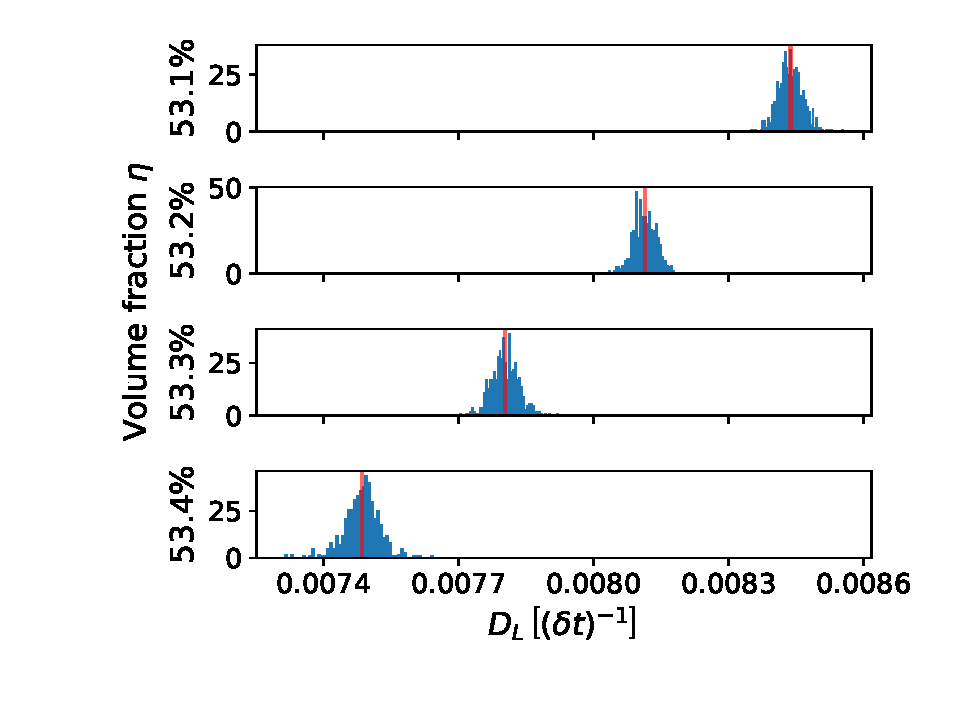
\includegraphics[width = 0.45 \textwidth]{diffusion_histogram_comparison.pdf}} \hspace{0.5cm}
\subfloat[Mean of the histograms with the uncertainty on the mean given by $\sigma_{\langle D \rangle} = \sigma_D/\sqrt{n}$ with n being the number of measurements included in the average.]{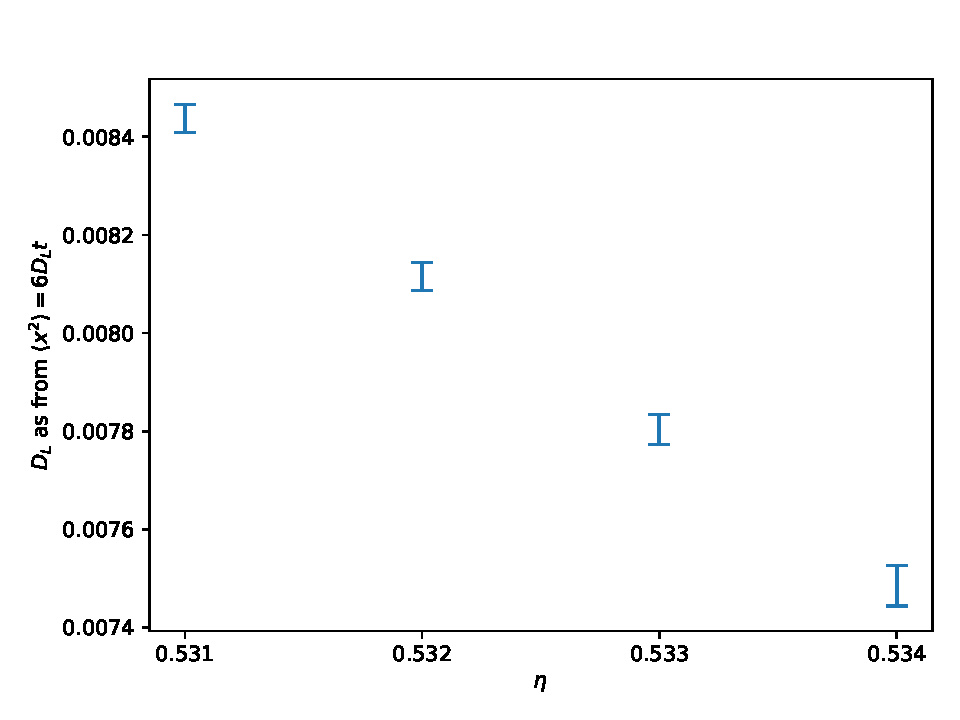
\includegraphics[width = 0.45 \textwidth]{diffusion_comparison.pdf}}  
\caption{Comparison of long time selfdiffusion constants at different volume fractions as histograms and their means with uncertainty.}
\label{fig:diffusion_comparison}
\end{center}
\end{figure}

The diffusion coefficents are important to know for comparsion between different systems. This importances is based on the idea that the fundamental mechanisms for nucleation and cluster growth do not vary between different hard sphere like systems, but are only scaled by the varying diffusion times. Furthermore their are theoretical predictions for the relationship of short time and long time diffusion, making it possible to compare experiments where the short time diffusion behaviour is better accesible with the ballistic simulations where only the long time diffusion constant is measurable.\\


As we see in \autoref{fig:diffusion_comparison} the diffusion constants can be measured with rather good precision with a relative standard deviation of $\sigma_D/D \approx 1\%$. Such it does not introduce large uncertainties when normalizing time related quantities by the diffusion time $\tau_{D} = D^{-1}$.

\section{Cluster growth}
\label{sec:Cluster growth}
Ounce the clusters reach a certain size they are expected to grow with new particles being attached to the surface at a constant rate leading to a growth with a proportionality of $N \propto t^3$ as shown in \autoref{eqn:constant_growth} where k is the assumed constant attachment rate, N is the number of particles in a specific cluster, A is the surface of the cluster, R is the radius of the cluster and $\rho_{solid}$ is the bulk density which is for large clusters a good approximation of the cluster density.\\

\begin{align}
\label{eqn:constant_growth}  
\begin{split}
\dot{N} &= k A \\
          & \; \; \, \vrule
  \begin{aligned}[t]
    \quad \text{with}  \quad  N &= \frac{4}{3} \pi R^3 \rho_{solid}\\
    \Leftrightarrow R &= \left( \frac{3 N }{4 \pi \rho_{solid} }\right)^{\frac{1}{3}} \, \text{,} \\
    \quad \text{and}   \quad A &= 4 \pi R^2 \\
    \Leftrightarrow A &= \left(\frac{4 \pi 3^2 }{\rho_{solid}^2} \right)^\frac{1}{3} N^\frac{2}{3} \, \text{,}\\
%    \quad \text{follows} \quad A &\propto N^\frac{2}{3} \\
  \end{aligned}\\
\frac{dN}{dt} &= k \left(\frac{4 \pi 3^2 }{\rho_{solid}^2} \right)^\frac{1}{3}  N^\frac{2}{3}\\
\end{split}
\hspace{1cm}
\begin{split}
%\Rightarrow \frac{dN}{dt} &= c' N^\frac{2}{3}\nonumber\\
%\vspace{0.25cm}\nonumber\\
& \!\!\!\!\!\!\!\!\! \text{From the bottom left side}\\
\Rightarrow& \quad dN \; N^{-\frac{2}{3}} = dt \; k \left(\frac{4 \pi 3^2 }{\rho_{solid}^2} \right)^\frac{1}{3}\\
          & \; \; \, \vrule
  \begin{aligned}[t]
    \quad \text{setting}  \quad  N(t=0) = 0\\
  \end{aligned}\\
\Leftrightarrow& \quad 3 N^{\frac{1}{3}} = k \left(\frac{4 \pi 3^2 }{\rho_{solid}^2} \right)^\frac{1}{3} t\\
\Leftrightarrow&  \quad N^{\frac{1}{3}} = k \left( \frac{4 \pi}{3 \rho_{solid}^2} \right)^\frac{1}{3} t
\end{split}
\end{align}  

As the systems are able to accomodate clusters up to a few hundred thousand particles and usually only one very large cluster is formed during a simulation, the attachment rate can be measured by a linear regression to the third root of the number of particles in the largest cluster over time. This is visualized for the trajectories at $\eta=0.532$ in \autoref{fig:cluster_growth_example}. The volume fraction $\eta=0.532$ is choosen arbitrarily.


\begin{figure}[h]
\label{fig:cluster_growth_example}
\centering
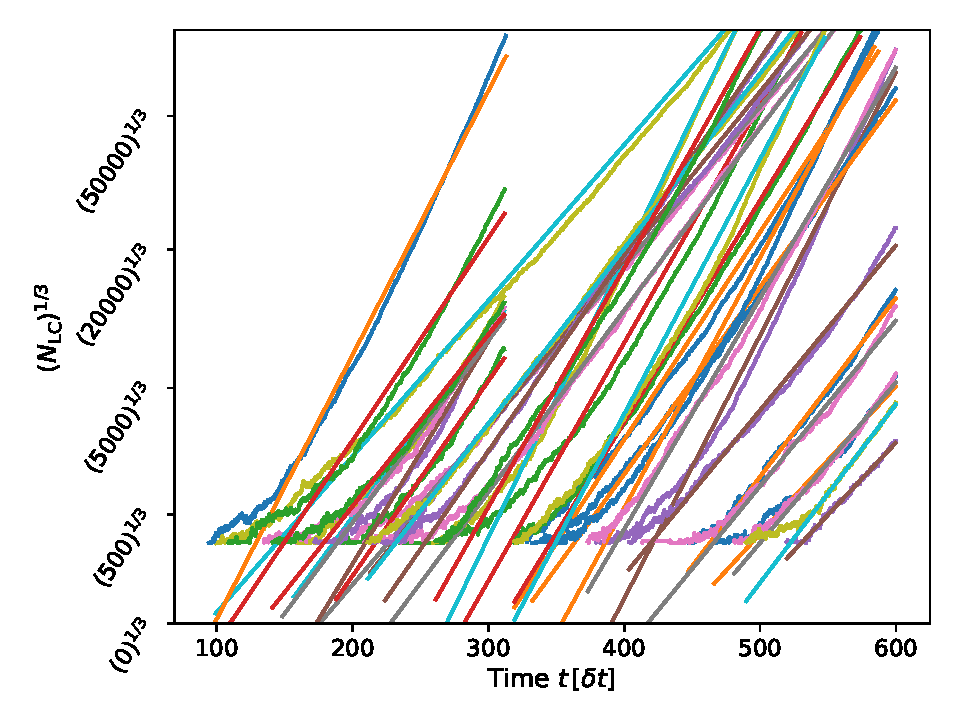
\includegraphics[width=0.7 \linewidth]{cluster_growth_example.pdf}
\caption{Trajectories of the third root of the number of particles within the largest cluster of a system over time. Clearly visible is the linear proportionality for which a linear regression is shown together with the data. The cut of some data sets at $t/\delta t \approx 300$ is due to the trepassing of the maximum walltime of the NEMO cluster. This means that the simulation of 20000 production steps yields a system time of $T/\delta t \approx 300$. Clusters present already in the first step would become to large in the next simulation intervall leading to a breach of the walltime limit due to the quadratic effort reuired for the q6q6 cluster finding routine. It can be assumed that clusters forming just around $t/\delta t \approx 300$ might not have been recognized due to this flaw. But as the number of trajectories concerning this is rather small the impact is not easy to reckognize when looking at the induction time distributions in \autoref{fig:induction_times}.}
\label{fig:cluster_growth_example}
\end{figure}

Subsequently the slopes of the linear regressions have been collected in histograms shown in \autoref{fig:constant_growth_rates}. As shown in \autoref{eqn:constant_growth} these slopes correspond to constant attachment rates with a dependence on the density within the cluster. As the densities of concern are very close to each other, they only introduce a relative difference of 0.5\% between the rates of lowest and highest volume fractions. Such we can neglect this dependence for the qualitative comparison.\\ 

\begin{figure}[h]
\begin{center}
\subfloat[Histograms of the slopes for the linear regressions to the largest clusters during the later constant growth process. The histograms are for $\eta=0.531,\;0.532,\;0.533,\;0.534$.]{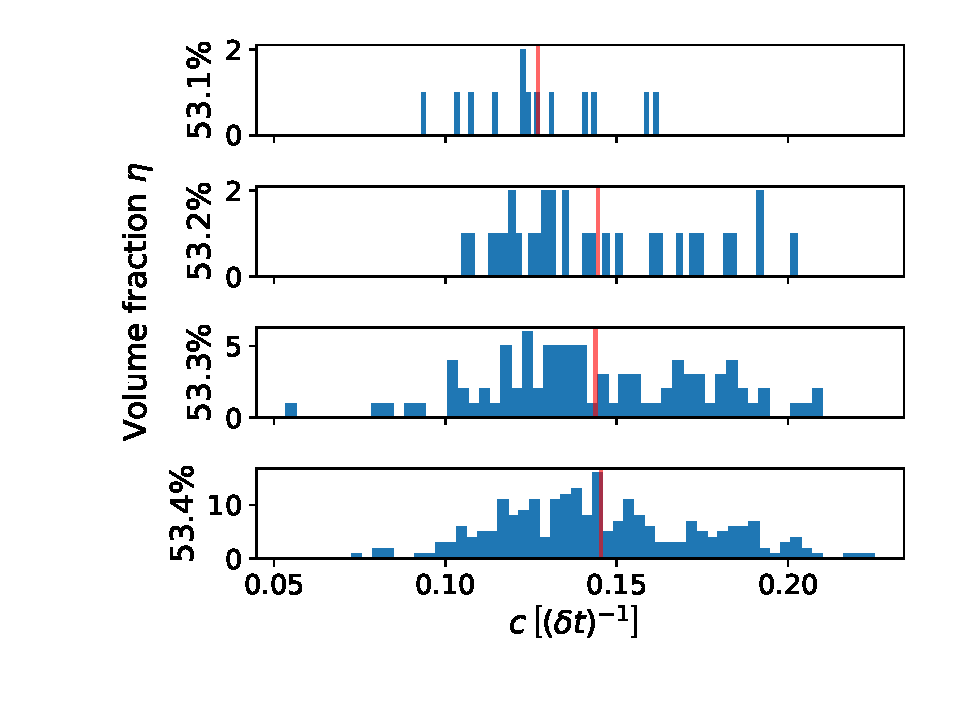
\includegraphics[width = 0.45 \textwidth]{const_growth_rate_histogram_comparison.pdf}} \hspace{0.5cm}
\subfloat[Mean of the histograms with the uncertainty on the mean given by $\sigma_{\langle c \rangle} = \sigma_c/\sqrt{n}$ with n being the number of measurements included in the average. \todo{is the standard deviation here more sensefull, as interest lays on the widht of the distribution not so much on the mean?}]{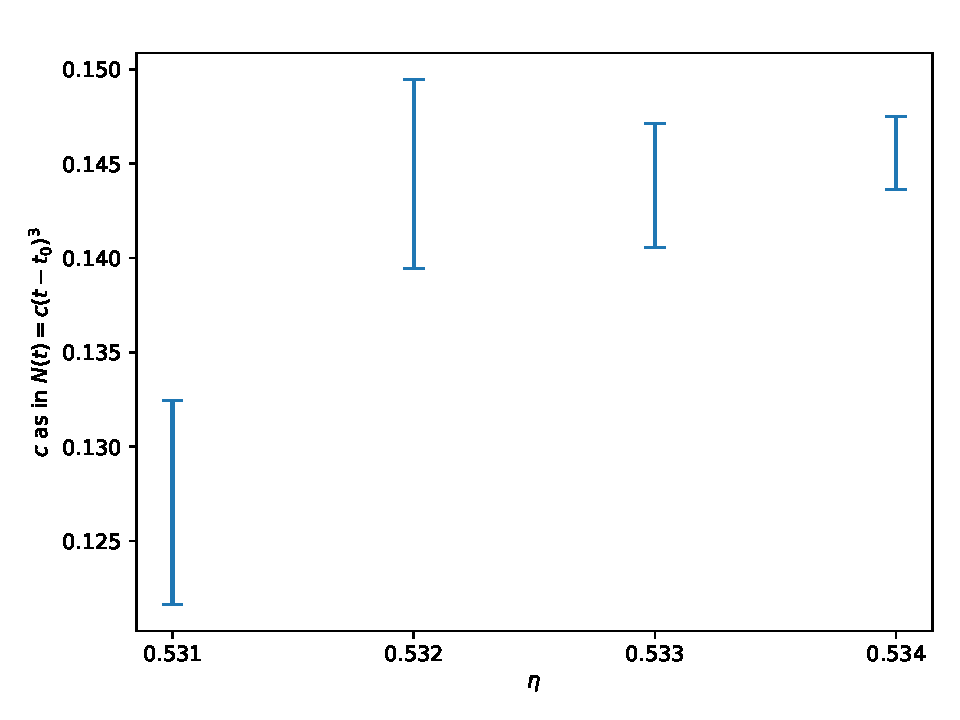
\includegraphics[width = 0.45 \textwidth]{const_growth_rate_comparison.pdf}}  
\caption{Comparison of growth rates in the constant attachement regime.}
\label{fig:constant_growth_rates}
\end{center}
\end{figure}

What we see from the histograms is that the distribution is rather spread out, but interestingly not signigicantly depending on the volume fraction. Except for $\eta = 0.531$ we find a smaller groth rate. A possible explanation for this behaviour could be that growth by heterogenous crystalization on the growing cluster surface, leading to a mean higher growth rate for higher volume fractions, is less likely for the lower volume fracitons. Either way due to the low statistics at the lowest volume fraction it is also possible that only a statistical fluctuation is seen. From the similarity of the growth rates we can deduce that the attachement of the particles to the cluster is a reaction controlled process. \todo{is this REACTION or diffusion controlled? And can we compare to literature in this case? In that case take up the densities} \\

As the diffusion constants vary from $D=0.0081|_{\eta = 0.532}$ to $D=0.0075|_{\eta = 0.534}$ they span a difference of about 7.5\%, but does that mean they are either reaction or diffusion controlled, or is their only nothing to see, as the uncertainty on the growth rate is also of the size 5 \% ?

\section{Tensor of Gyration properties}
\label{sec:tog}
The tensor of gyration is a very usefull tool as it describes the second moments of the position distributions. Such it comprises information about the spatial extent in all three dimensions, from which we can derive quantities as the radius of gyration, asphericity or anisotropy which will be defined following the definitions in the wikipedia \todo{either find an other source or cite it correctly}.\\

The tensor of gyration is defined by \autoref{eqn:tensor_of_gyration}.
\begin{align}
\label{eqn:tensor_of_gyration}
&S_{mn}=\frac{1}{N} \sum_{i=1}^{N} r^{(i)}_m r^{(i)}_n\\
\label{eqn:center_of_mass}
&\text{with} \quad \sum_{i=1}^{N} \vec{r}^{(i)} = 0
\end{align}

As described by \autoref{eqn:center_of_mass} the matrix $S_{mn}$ is calculated in the center of mass frame for particles with the same mass. Furthermore the tensor of gyration can be diagonalized, with the three Eigenvalues $\lambda_1^2$, $\lambda_2^2$ and $\lambda_3^2$. The cartesian system thereby is choosen such that $\lambda_1^2 \leq \lambda_2^2 \leq \lambda_3^2 $. These Eigenvalues correspond to the spatial extents of the cluster within the cartesian system in which the tensor of gyration becomes diagonal. From these three Eigenvalues the quantities defined in \autoref{eqn:tog_quantities1} - \ref{eqn:tog_quantities4} are common to characterize clusters of particles.

\begin{align}
\label{eqn:tog_quantities1}
\text{(squared) Radius of gyration:} \quad &R_G^2 = \sum_{i=1}^3 \lambda_i^2\\
\label{eqn:tog_quantities2}
\text{Asphericity:} \quad &b = \lambda_3^2 - \frac{1}{2}(\lambda_1^2+\lambda_2^2)\\
\label{eqn:tog_quantities3}
\text{Acylindricity:} \quad &c = \lambda_2^2 - \lambda_1^2\\
\label{eqn:tog_quantities4}
\text{Relative shape anisotropy:} \quad &\kappa^2 = \frac{b^2 + \frac{3}{4} c^2 }{R_G^4} =  \frac{3}{2} \frac{ \sum_{i=1}^3 \lambda_i^4 }{\left(\sum_{i=j}^3 \lambda_j^2 \right) ^2 } - \frac{1}{2}
\end{align}

For better understanding of the shape descriptors mentioned before, we can have a more detailed look at their interpretation:

\begin{description}
\item[Radius of gyration $R_G$:] \hfill \\ An averaged radius of the structure.
\item[Asphericity b:]\hfill \\ The difference of the largest extrent with an average of the two smaller extents. 
\item[Acylindiricty c:] \hfill \\ The difference of the smaller extents
\item[Relative shape anisotropy $\kappa^2$:] \hfill \\ A sum of the asphericity and the acylindricity normalized by the radius of gyration to obtain a dimensionless quantitiy between 0 and 1.
\end{description}



To spot possible correlations between cluster shape and growth rates at early or late stages as well as correlations concering the induction time the three quantities \autoref{eqn:tog_quantities1} - \ref{eqn:tog_quantities4} derived from the tensor of gyration have been first plotted versus the cluster size when the quantity was measured to make them comparable. As the number of particles in the cluster is not monotonously increasing, the depicted quantity is not a function anymore. Either way it makes sense to show the data in this form, as we expect that we can compare clusters best at a defined number of particles. Furthermore the number of particles, as well as the quantities can span many orders of magnitude making logarithmic scales useful.\\
To finally highlight correlations between the aforementiond growth related scalar quantities and the tensor of gyration quantities, the single trajectories have been coloured by the corresponding magnitude of the scalar quantity. A large overview produced by this procedure is given in \autoref{fig:tog_overview} for the nucleated trajectories at $\eta=0.534$.

\begin{figure}[!h]
\centering
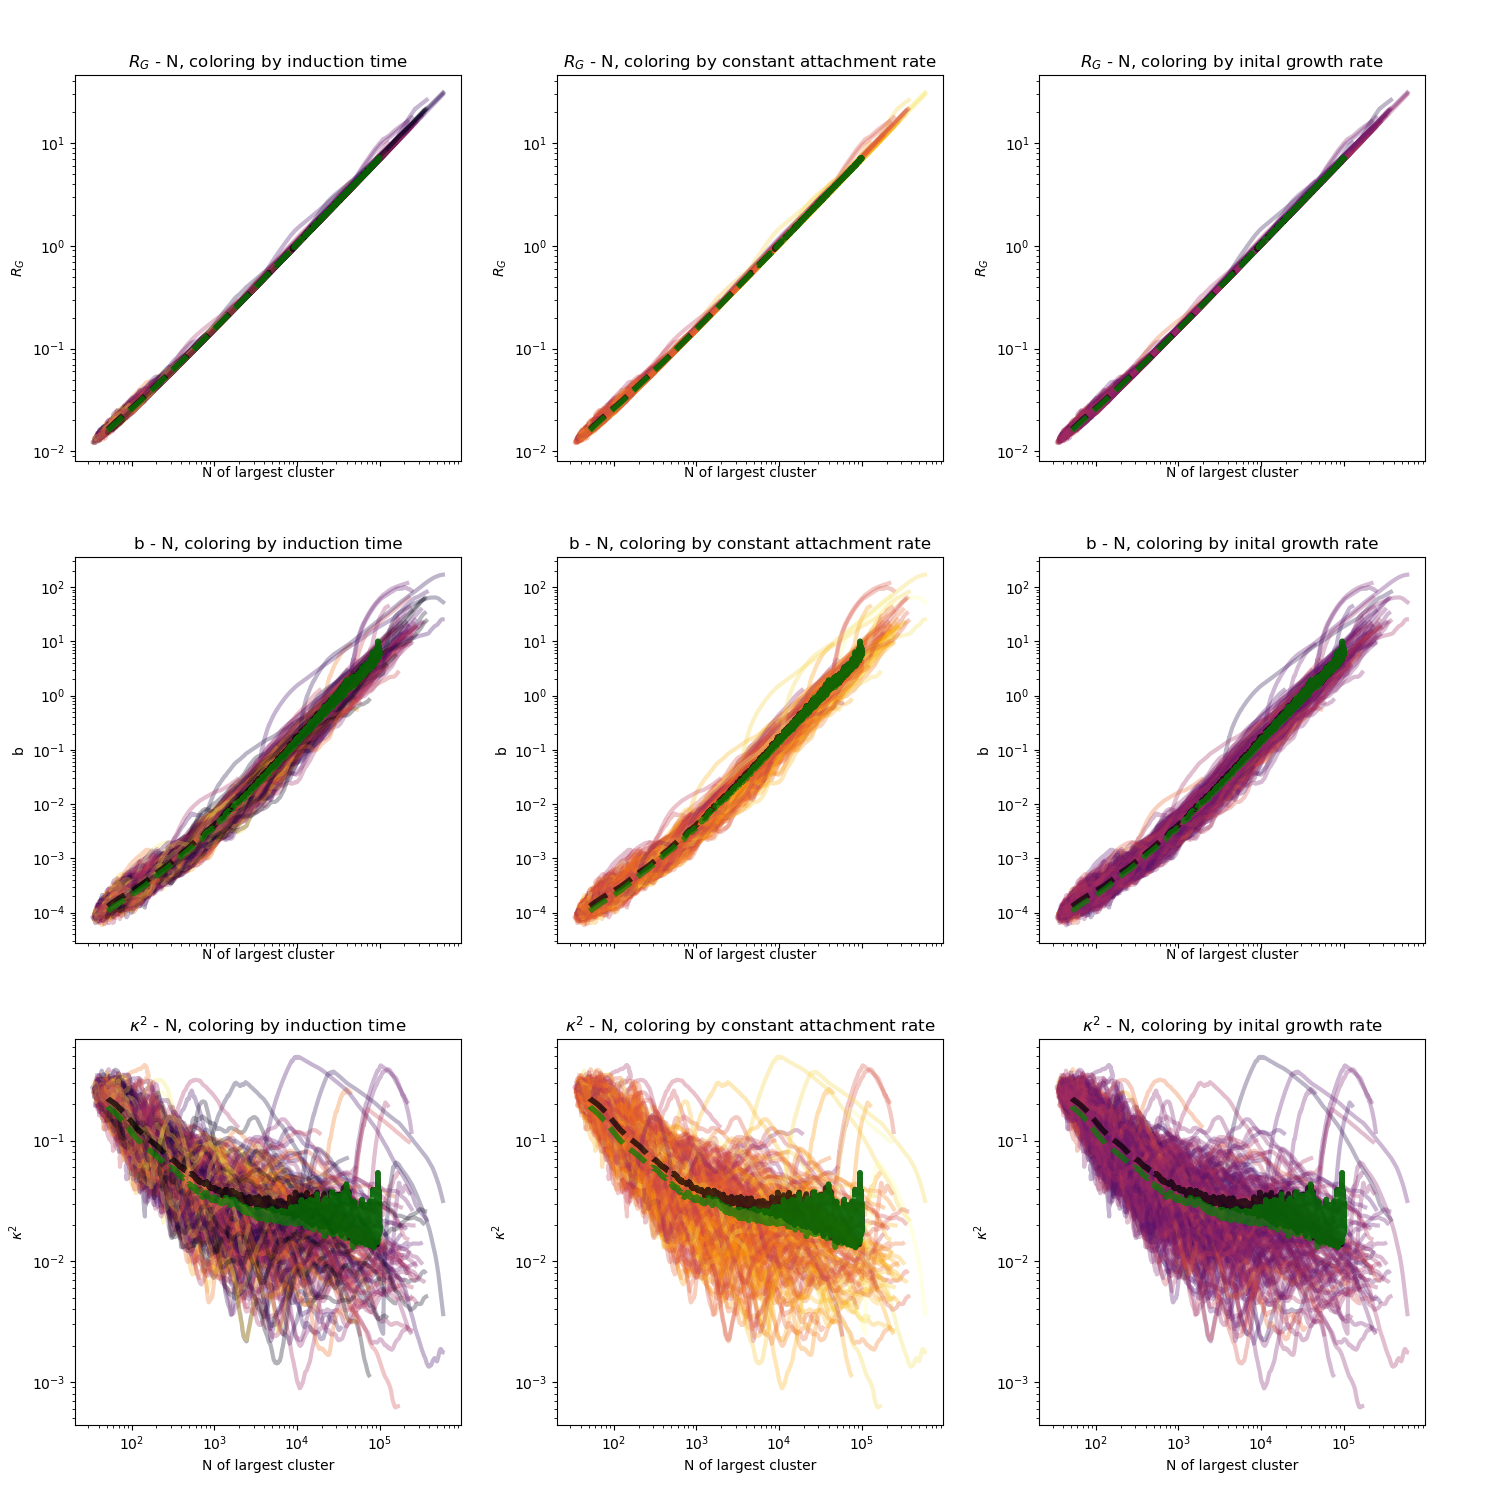
\includegraphics[width=0.8 \linewidth]{Series_534_corrolation.png}
\caption{Overview of the cluster shape describing quantites radius of gyration ($R_G$), asphericity (b) and anisotropy ($\kappa^2$), depending on the size of the cluster. The colouring depicts the scalar quantities induction time, constant attachment rate and inital growth rate.}
\label{fig:tog_overview}
\end{figure}

With the overview it was tried to capture different characeristic features of the cluster growth. The induction time is choosen, because clusters nucleating shortly after the quench might start with a  less organized structure which could lead to a higher asphericity at early times.\\ 

Also a possible idea would be that clusters starting with a slow growth at the beginning might be less structured, as this could make attachement of new particles harder and melting more likely. For quantifying the inital growth rate, an exponential function has been fitted to the data up to a cluster size of 500 particles. The growth rate within the exponential function is taken as measure on how swift the nucleation process works from the precursor to the growing crystal.\\

The third scalar quantity is the attachement rate of the cluster at later times. As this attachment rate might be linked to the number of defects within the crystal or other structural properties like the present crystal strucure or purity of the crystal it was also thought to be corrolated to easily accesible properties of the cluster like the shape descriptors.\\

But from the overview we get no obvious sign that there are any correlations between cluster shape and growth rates or between cluster shape and the induction time. Because of that no deeper analysis is done, but instead we conclude that by this superficial analysis we cannot relate the shape descriptors of the cluster to growth or structural properties.\\

\section{Autocovariance functions ( largest cluster, p(n,t) ) }
\label{sec:acf}
\todo{talk about if this is usefule in any way.}

The autocovariancefunction (ACF) of the largest cluster contains information about how long a single cluster persists as the largest cluster within the volume, as flucutations of clusters at different points of the volume are expected to be independent of each other, the size fluctuation of a distinct cluster should be corroloated in time . (Except if we think about the modes within the fluid encompassing not only local areas...)\\

The autocovariance function is defined by \autoref{eqn:definition_acf}, where $N_{lc}(t)$ is the number of particles in the largest cluster at time t, $\langle N_{lc} \rangle_t$ is the corresponding average over time, thus $X(t)$ describes the deviations from the average. The autocovariance function furthermore is normalized by ${ \langle X^2  \rangle }$ which can be identified as the variance of the data. With this normalization $ACF(\tau=0) = 1 $.

\begin{align}
\label{eqn:definition_acf} 
ACF(\tau)=\frac{ \langle  X(\tau)-X(0) \! \: \rangle } { \langle X^2  \rangle }\\  
\text{with } X(t)=N_{lc}(t)- \langle N_{lc} \rangle_t 
\end{align}

The calculation is performed on the time resolved largest cluster within a measurement. As the ACF is supposed to give insight to the fluctuations of clusters in the metastable fluid only measurements that did not nucleate or at least involved only little cluster growth were used for the ACF in \autoref{fig:acf}.  



\begin{figure}[h]
\begin{center}
\subfloat[$\eta = 0.531$]{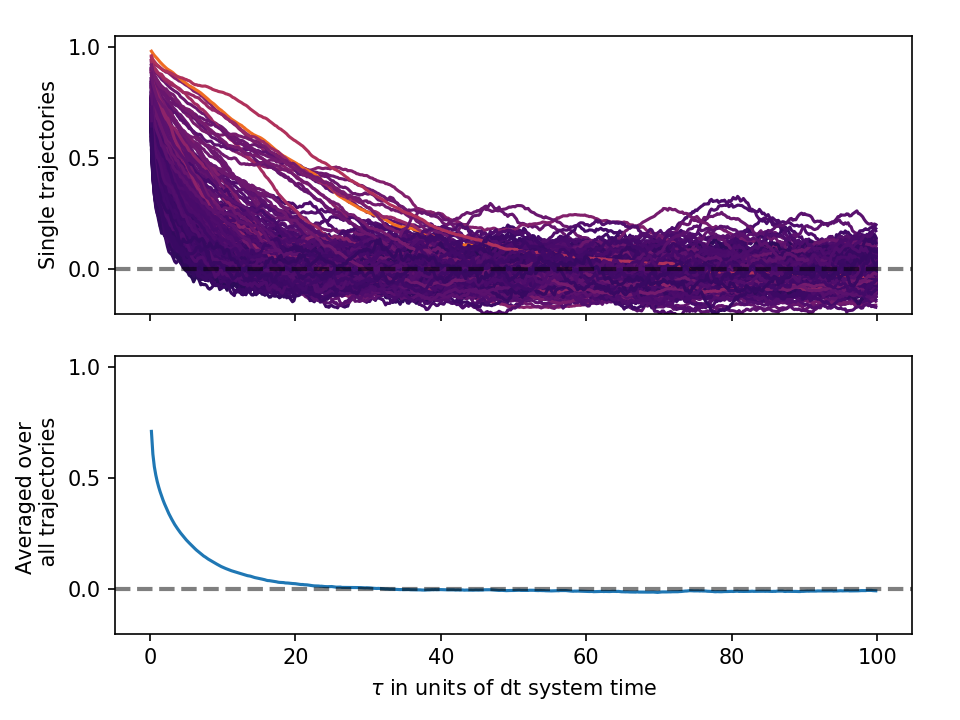
\includegraphics[width = 0.4 \textwidth]{acf_lc_531.png}} \hspace{0.5cm}
\subfloat[$\eta = 0.532$]{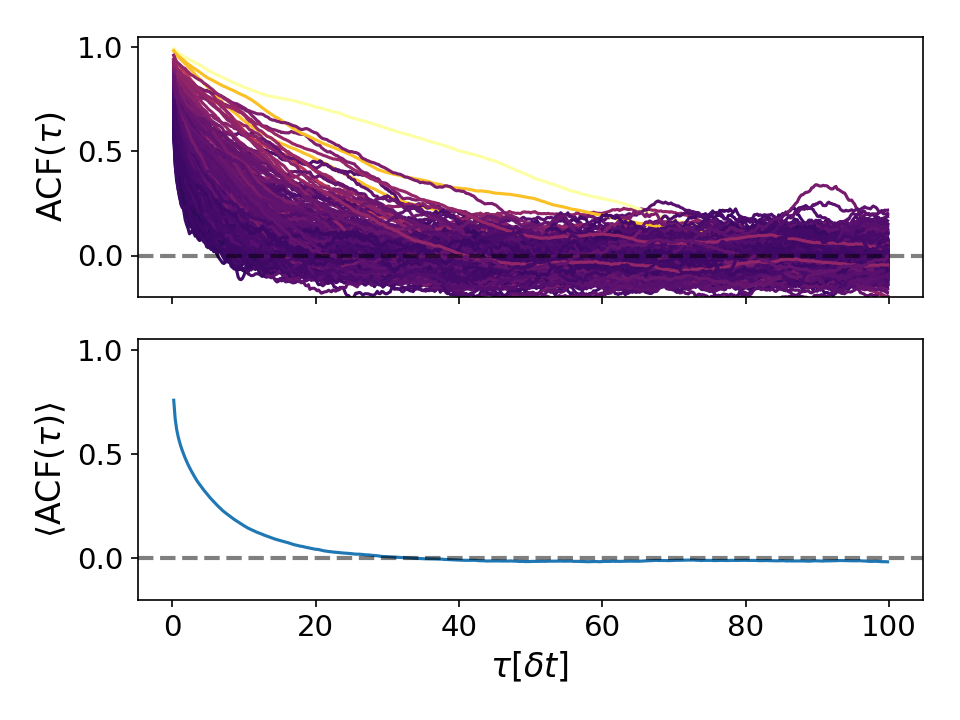
\includegraphics[width = 0.4 \textwidth]{acf_lc_532.png}} \\
\subfloat[$\eta = 0.533$]{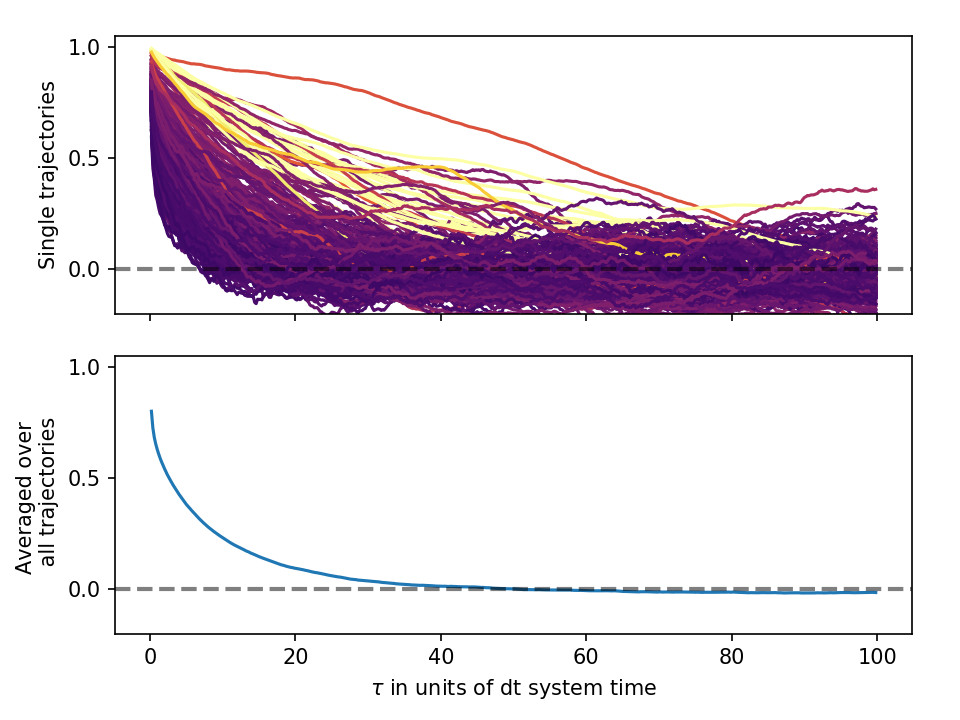
\includegraphics[width = 0.4 \textwidth]{acf_lc_533.png}} \hspace{0.5cm}
\subfloat[$\eta = 0.534$]{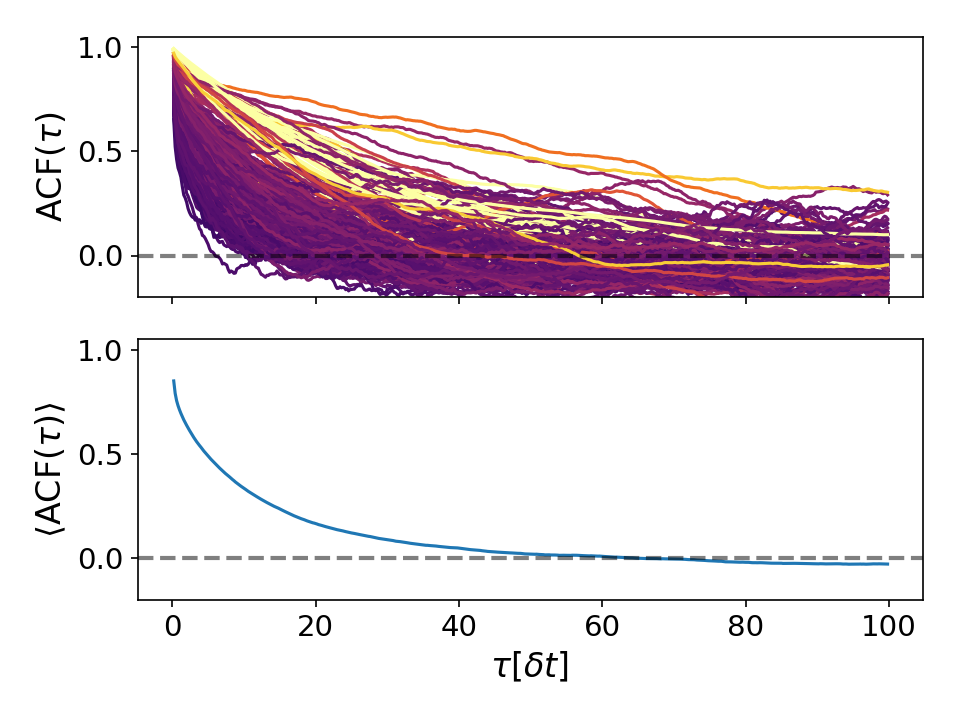
\includegraphics[width = 0.4 \textwidth]{acf_lc_534.png}} \\
\caption{Comparison of autocovariance functions in the metastable fluid. The colouring corresponds to the largest cluster present over the whole simulation time. The lightest colour indicate therby a largest cluster of more than 500 hundred particles which can more or less also be called nucleated, but these are rare in the given selection and such the data represents the metastable fluid still rather good.}
\label{fig:acf}
\end{center}
\end{figure}

From the autocovariance functions we see that stuructural flucutation seen as clusters persist for longer times at higher volume fractions. From the colorring as well as from the cluster distributions we can also conclude that the fluctuations tend to be larger at higher volume fracitons.

\section{Nuclection time dilemma}
\label{sec:nucleation_times}

To later on calculated induction times or average nucleation times, we will require a definition of when a crystal is called nucleated. This means we have to define from which point a cluster is not merely a unstable fluctuation within the liquid anymore, but instead becomes a stable solid crystaline phase.\\ 
In the literature many concepts are used. For example a cluster can be defined as crystaline soon as its of the critical size, calculated by CNT or by doing a comitter analysis. An other possibility often used is to rewind the trajectory soon as a clearly stable crystal is found, up to the point when the crystal clusters size more or less vanishes. A further approach is to fit the growth during later times and extrapolate it to the time when the cluster vanishes.\\

All these definitions differ more or less only by a delay $\Delta_{\tau}$ which is a distribution of times holding the information of how long it takes for varying clusters to pass from the first criterion to the next.\\
For example we can take as a first point the time when a cluster, known to crystalize at later times, cannot be differentiated anymore from any other structural fluctuation in the liquid, i.e. when the size of the cluster falls below some threshold given by the size of clusters regularly present in a given volume.\\
The second point we can set by either the critical size of CNT or by some other criterion when we are sure that the cluster has stabilized and will only continue to grow.\\
At the first of these two points, the fluctuation leading to the crystalization occurs but it would not be possible to tell yet if this precursor melts or continues to grow, while at the second point the crystal is stable. Such the first might be called a precursor nucleation and the second crystal nucleation. Between these two points we find the time difference to be the time it takes for the precursors to form a stable crystal. This includes also that some precursors might loiter for awhile before forming the stable phase while other pass this gap rather directly.\\

When calculating a mean induction time, the delay $\Delta_{\tau}$ propagates also to the final result and as it is a stochastic distribution also its higher moments are propagated leading to a smaller precision. This afterall only means that the induction time depends on the definition of crystalization and they are only roughly comparable.\\ 
In \autoref{fig:induction_distributions} three distirbutions with varying definitions of the induction time are visualized.

\begin{figure}[!h]
\centering
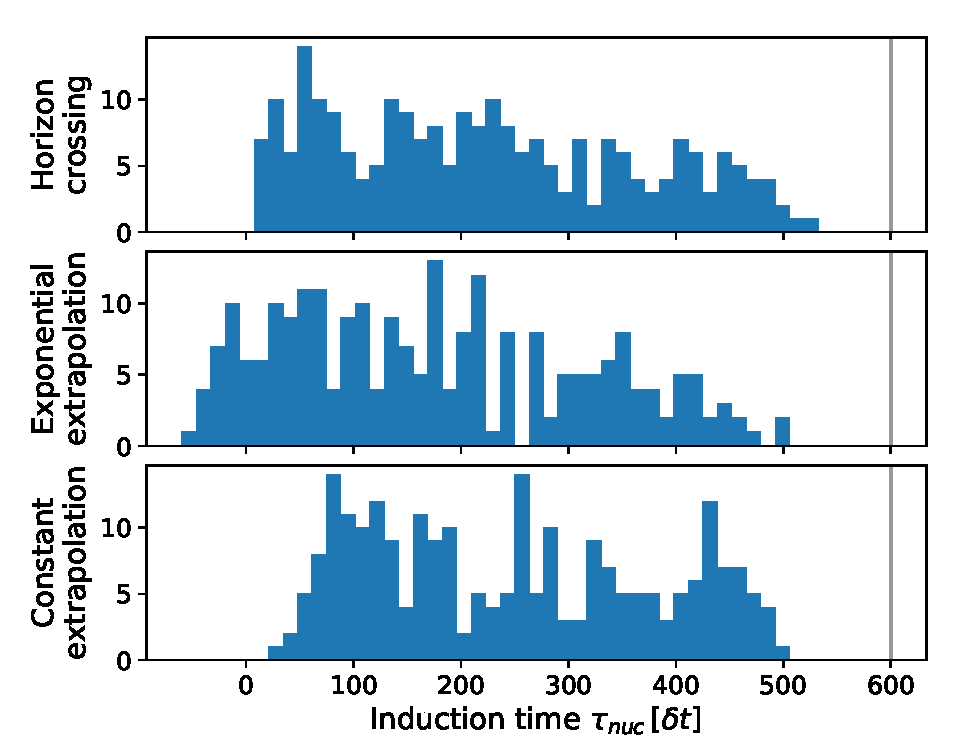
\includegraphics[width=0.7 \linewidth]{varying_induction_time.pdf}
\caption{Induction time distribution obtained by different definitions. While the two methods using extrapolation seem to have the two effects of smearing the signal as well as shifting them, the method of defining the nucleation as the time when the largest cluster is last below the horizon of fluctuations seems to return the most accurate and precise distribution. The final simualtion time is mrked by the grey line. As clusters require some time to be clearly recognised as crystals no nucleation are seen towards the end of the simualtion intervall. To counteract this we will truncate the distribution in the following analysis such that this does not have an impact on the final result.}
\label{fig:induction_distributions}
\end{figure}

The three methods explicitly used here are given by the following:
\begin{description}
\item[Horizon crossing]{The time of nucleation is obtained by following the trajctory of the largest cluster within a system after it clearly nucleated back to the point where it was the last time at the average largest cluster of the metastable fluid without stable cluters. The name horizon crossing refers therby to the idea that fluctuations of the largest cluster in the metastable fluid are more or less independent fluctuations. This comes by the fact that the large fluctuations of the system alternate at being the largest one, and such the largest fluctuations is not bound locally and the fluctuations becomes independent events. On the other side an extraordinary fluctuation will be seen for a longer period of time as the largest cluster, and thus the corresponding flucutuations are not independent in time. The crossing of the trajectory below this horizon where it cannot be followed any longer is meant by the name.}

\item[Exponential extrapolation]{For this method an exponential growth is fitted to the largest cluster data up to N<500. Extrapolating to smaller times makes it possible to evaluate when the exponential crossed 10 particles, which is then taken as the induciton time. The method tends to find negative induction times that are not physical.}

\item[Constant extrapolation]{The name refers to the constant attachment rate found at later times for the cluster growth. It can be extrpolated to earlier times until the cluster has completly vanished i.e N=0. As the constant attachement rate is higher than the inital growth rate this method returns too large induction times.}
\end{description}

As can be seen the horizon crossing method returns a rather smooth distribution that also roughly can be approximated by an exponential decay that is expected for a constant nucleation rate as will be shown in \todo{put in the correct section or equation}.\\


%\subsection{induction time by critical cluster from cnt}
%-r\_crit calc and induction time distribution

%\subsection{inudction time by constant growth extrapolated to zero}
%-linear regression and distribution of constant growth rates\\
%-induction time ditribution

%\subsection{induction time by exponential fit}
%- maybe procedure\\
%- distribution rates\\
%- distribution inducion times

%\subsection{induction time by fluctation horizon crossing}
%- non locality of fluctuations -> acf?\\
%- sensefull to use the data until it vanishes\\
%- induction time distribution\\
%- discuss the delay distirbution (precursor structuring time)\\ 
%- evaluation of an simple induction time or rate by cnt next chapter

\section{Induction time by exponential distribution}
\label{sec:induction_times}
Estimating the induction time of the hard sphere nucleation has been done over the previous two decades multiple times by experimentalists and theorists. The employed procedures vary \todo{do they vary or are they just the mean every time? Well the experimentalists use the point when the whole sample crystalizes.} between experimentalists and theorists as the experimentalists often have access to very large systems but wihtout knowing all positions at all times, while the theorists mostly have smaller system in simulations with the adavantage of being able to access all particle positions and in case of simulations probing the dynamics also at all times.\\

Furthermore theorists have used simple approaches like the average induction time which has involves the constraint that all trajectories of an ensemble are required to have nucleated. This is very suitable and simple for systems at large volume fractions as for them all simulations of an ensemble might be calculated up to nucleation. At lower volume fractions this becomes more and more unfeasible due to the steep increase of the induction time.\\

To cirumvent this problem we will define the nucleation rate in the following differently without requiring all simualtions to nucleate. In fact we can also show that the uncertainty of the induction time obatained from the data is not signifiantly reduced anymore for measurements longer than the induction time.\\     

\subsection{CNT expectation the induction time distribution}
\label{sec:induction_time_expectation}
In \autoref{sec:CNT} we introduced Classical nucleation theory and its constant nucleation rate depending on the barrier height in the free energy landscape. Even if there are signs that CNT is not appropriate for describing nucleation process perfectly, we will use its prediction of a constant nucleation rate as an assumption to define such a constant scalar nucleation rate.\\

As also mentioned before, in the discussion of the system sizes (\autoref{sec:system_choice}), the induction time of a system depends on the volume under consideration and such the nucleation rate is commonly defined as a nucleation rate density $k$.\\ 
Considering now the simualtions we can describe them as a total of $m$ volumes with a size of $V_{box}$.  Further we can define the number of boxes in which a nucleation occured as $n(t)$ and exclude these from the further simulation.\\

In this case the total nucleation rate $ \dot{n} $ can be written by \autoref{eqn:nuc_rate} from which in the continous limit of an infinte number of different simulations we can deduce the expected induction rate.

\begin{align}
\label{eqn:nuc_rate}
\dot{n} &= (m - n(t))V_{box}k\\
\Leftrightarrow \frac{\dot{n}}{m} &= (1 - \frac{n(t)}{m})V_{box}k\\
 &  \text{in the limit } m \rightarrow \infty \nonumber\\
\Leftrightarrow \frac{n(t)}{m} &= 1 - \exp\left( -V_{box} k t \right)\\
 &  \text{defining } \tau = (V_{box} k)^{-1} \nonumber\\
\label{eqn:nuc_rate_result}
\Leftrightarrow \frac{\dot{n}(t)}{m} &= \frac{1}{\tau} \exp\left( \frac{-t}{\tau} \right) 
\end{align}

The final result in \autoref{eqn:nuc_rate_result} is the well known stochastic exponential distribution. As the expectation value of the exponential distribution is given by its parameter $\tau$ the common approach of using the mean induction time when all simulations have nucleated yields an accuracte result and precision can be obtained by taking a large number of simulations.\\


\subsection{Maximum likely estimator of induction time}
\label{sec:ml_estimator}
In case the simulation time is not feasible we instead will have to deal with truncated exponential distributions. For this we can use Maximum likelihood estimators. The derivation follows \todo{cite the statistics paper}.\\

Maximum likelihood estimators are based on the idea that we can write down the expression of the total probability called likelihood $\mathcal{L}$ for a given set of measurements $x_i$ depending on parameters of the assumed underlying distribution. For the exponential distribution parametrized by the characteristic decay rate $\kappa$ this is given by \autoref{eqn:exponential_product}.

\begin{align}
\label{eqn:exponential_product}
\mathcal{L}(\kappa) = \prod_{i=1}^N p(x_i) = \prod_{i=1}^N \kappa^N \exp\left( - \kappa x_i \right ) 
\end{align}

During the process we try to find the maximum of this product. To simplify this product and also to evade overflow problems on floating point machines, the logarithm of the likelihood is used and maximized yielding the same parameters because the logarithm is a monotonic function and thus does not shift the extrema.\\
The maximum probability can then be found by usual means of analysis executed in \autoref{eqn:exponential_maximization}.

\begin{align}
\label{eqn:exponential_maximization}
& 0 \stackrel{!}{=} \left. \frac{\partial \log(\mathcal{L})}{\partial \kappa} \right|_{\kappa=\hat{\kappa}}\\
\Leftrightarrow \qquad  &0 = \left. \frac{\partial}{\partial \kappa} \left( N \log(\kappa) - \kappa \sum_{i=1}^N t_i \right)  \right|_{\kappa=\hat{\kappa}} \\
\Leftrightarrow \qquad &0 = \frac{N}{\hat{\kappa}} - \sum_{i=1}^N t_i \\
\Leftrightarrow  \qquad & \!\!\!\!\!\!\!\!\: \hat{\kappa}^{-1} = \frac{1}{N} \sum_{i=1}^N t_i  
\end{align}

Such we have found that the maximum likelihood estimator of $\kappa$ for a set of samples drawn from an exponential distribution is given by the inverse arithmetic mean of the samples. This result is neither new nor surprising but is shown to illustrate how the method of maximum likelihood works. In the following we then show how to handle censored and truncated distribtuions by the maximum likelihood method.\\
Both terms in this context refer to sets of samples that are incomplete in the sense that they only include samples up to some threshold $t_i < T$. In the case of truncated distributions the number of samples larger than this threshold is unknown while for the censored distribution the number of samples is known. Taking the example of time consuming nucleation events in computer simulations we are in the case of censored distributions, as the total number of simulation boxes is known but the simulation is stopped at some point when enough nucleations have been collected and such the number of samples that would have nucleated at later times is known. The probability of an event after the end of the simulation is given by \autoref{eqn:prob_t_larger_T}.
\begin{equation}
\label{eqn:prob_t_larger_T}
p(t_i>T) = \int_T^{\infty} \kappa \exp(-\kappa t) dt = \exp(-\kappa t) 
\end{equation}
The probability distribution not only below the threshold but also above can then be written as in \autoref{eqn:pdf_censored}.
%\begin{align}
%\begin{split}
%f(t) = 
%\end{split}
%\begin{split}
%\hspace{-5cm}
%\begin{cases}
%\kappa \exp(-\kappa t) & t < T\\
%\exp(-\kappa T) & t \geq T\\ 
%\end{cases}
%\end{split}
%\end{align}
\begin{align}
\label{eqn:pdf_censored}
f(t) = 
\begin{cases}
\kappa \exp(-\kappa t) & t < T\\
\exp(-\kappa T) & t \geq T\\ 
\end{cases}
\end{align}


In the simulation we can split up the number of boxes $N$, into $n$ boxes where a nucleation event was found, and $m = N -n$ others where no nucleation event was spotted during the simulation time $T$.\\
Further we have to account for the fact that the samples without distinct times are indistinguishable. This is done by weighting them with the number of possible permuations given by the binomial prefactor $\binom{N}{m}$. The whole expression is then given in \autoref{eqn:ml_censored_exponential} and the extremum of the likelihood function is evaluated in the subsequent reformulation.

\begin{align}
\label{eqn:ml_censored_exponential} 
\mathcal{L}(\kappa) & = \left. \binom{N}{m} \;  \kappa^n \; \exp(- \kappa \sum_{i=1}^n t_i) \;  \exp(-\kappa T)^m \quad \right| \left.\frac{\partial \log ( ... )}{\partial \kappa} \right|_{\kappa=\hat{\kappa}} \\
\Leftrightarrow \quad\log ( \mathcal{L}(\kappa)) & = \left.\log\binom{N}{m}  + n \log ( \kappa) - \kappa \sum_{i=1}^n t_i - m \kappa T \quad \right| \left. \frac{\partial(...)}{\partial \kappa} \right|_{\kappa=\hat{\kappa}} \\
\Leftrightarrow \:\! \frac{\partial \log ( \mathcal{L}(\kappa))}{\partial \kappa} & = \left. \frac{n}{ \kappa} - \sum_{i=1}^n t_i - m  T \quad \right|_{\kappa=\hat{\kappa}}\\ 
 & \; \; \, \vrule
  \begin{aligned}[t]
      \raisebox{0.9cm}{ \makebox[1cm]{}} \raisebox{-0.5cm}{ \makebox[0.5cm]{}}  \text{with } \frac{\partial \log ( \mathcal{L}(\hat{\kappa})  )}{\partial \kappa}  \stackrel{!}{=} 0  \\
  \end{aligned} \nonumber\\
\Leftrightarrow \qquad\qquad \;\; \:\! 0 &= \frac{n}{ \hat{\kappa}} - \sum_{i=1}^n t_i - m  T \quad\\
\label{eqn:ml_censored_exponential_final}
 \Leftrightarrow \qquad\quad  \;\: \hat{\kappa}^{-1} &= \frac{1}{n} \left(  \sum_{i=1}^n t_i + m T \right)
\end{align}

%\begin{align}
%\label{eqn:ml_censored_exponential} 
%\left. \frac{\partial \log ( \mathcal{L}(\kappa)  )}{\partial \kappa}   \right|_{\kappa=\hat{\kappa}} & \stackrel{!}{=} 0  \\
%& \qquad \text{with} \quad \mathcal{L}(\kappa) =\binom{N}{m} \;  \kappa^n \; \exp(- \kappa \sum_{i=1}^n t_i) \;  \exp(-\kappa T)^m  \\
%\Leftrightarrow \qquad \qquad 0 &=  \left. \frac{\partial }{\partial \kappa} \log \left(  \binom{N}{m} \;  \kappa^n \; \exp(- \kappa \sum_{i=1}^n t_i) \;  \exp(-\kappa T)^m  \right)  \right|_{\kappa=\hat{\kappa}}\\
%\Leftrightarrow \qquad\qquad 0 &=  \left. \frac{\partial }{\partial \kappa} \left( \log\binom{N}{m}  + n \log ( \kappa) - \kappa \sum_{i=1}^n t_i - m \kappa T \right)  \right|_{\kappa=\hat{\kappa}}\\
%\Leftrightarrow \qquad\qquad 0  &=  \left. \frac{n}{ \kappa} - \sum_{i=1}^n t_i - m  T \quad \right|_{\kappa=\hat{\kappa}} \\
%\label{eqn:ml_censored_exponential_final}
%\Leftrightarrow \qquad \qquad \!  \hat{\kappa} &=  \left( \frac{m}{n} T + \sum_{i=1}^n t_i \right)^{-1} 
%\end{align}


%\begin{align}
%\label{eqn:ml_censored_exponential} 
%\left. \frac{\partial \log ( \mathcal{L}(\kappa)  )}{\partial \kappa}   \right|_{\kappa=\hat{\kappa}} & \stackrel{!}{=} 0  \\
%& \qquad \text{with} \quad \mathcal{L}(\kappa) =\binom{N}{m} \;  \kappa^n \; \exp(- \kappa \sum_{i=1}^n t_i) \;  \exp(-\kappa T)^m  \\
%\left. \frac{\partial \log ( \mathcal{L}(\kappa)  )}{\partial \kappa}   \right|_{\kappa=\hat{\kappa}}  &= \left. \frac{\partial }{\partial \kappa} \log \left(  \binom{N}{m} \;  \kappa^n \; \exp(- \kappa \sum_{i=1}^n t_i) \;  \exp(-\kappa T)^m  \right)  \right|_{\kappa=\hat{\kappa}}  \\
%\Leftrightarrow \left. \frac{\partial \log ( \mathcal{L}(\kappa)  )}{\partial \kappa}   \right|_{\kappa=\hat{\kappa}}  &= \left. \frac{\partial }{\partial \kappa} \left( \log\binom{N}{m}  + n \log ( \kappa) - \kappa \sum_{i=1}^n t_i - m \kappa T \right)  \right|_{\kappa=\hat{\kappa}}   \\
%\Leftrightarrow \left. \frac{\partial \log ( \mathcal{L}(\kappa)  )}{\partial \kappa}   \right|_{\kappa=\hat{\kappa}}  &= \frac{n}{ \hat{\kappa}} - \sum_{i=1}^n t_i - m  T \quad \\
% & \; \; \, \vrule
%  \begin{aligned}[t]
%    \quad \text{with } \left. \frac{\partial \log ( \mathcal{L}(\kappa)  )}{\partial \kappa}   \right|_{\kappa=\hat{\kappa}}  \stackrel{!}{=} 0 
%  \end{aligned}\\
%\label{eqn:ml_censored_exponential_final}
%\Leftrightarrow \quad \,  \hat{\kappa} &=  \left( \frac{m}{n} T + \sum_{i=1}^n t_i \right)^{-1} 
%\end{align}

The final line \autoref{eqn:ml_censored_exponential_final} is the estimator of the decay rate of the censored exponential distribution. It is used for the estimation of induction times to compare with other published results in the next sections.
%The aforementioned truncated distribution is not used wihin this thesis but for completness the result is still mentioned. The distribution of the truncated exponential distirbution is given by \autoref{eqn:truncated_exponential_distribution}.
%\begin{equation}
%\label{eqn:truncated_exponential_distribution}
%p(t) = \frac{\kappa \exp(-\kappa t)}{1-\exp(-\kappa T)}
%\end{equation}
%It differs only by the normalization factor as all known sample lay within the measurement intervall.
\subsection{Monte Carlo uncertainty estimaion}
\label{sec:mc_uncertainty}
Having found the estimator the next question is what is its uncertainty, i.e what is the distribution of $\kappa$. Eventhough corresponding literatur on analytic expresssions of the distribution exist the complexity becomes inappropriate for the task at hand. We will follow instead a Monte Carlo method proposed for example in the book Numerical Recipes \todo{cite numerical recispes} to find the uncertainty of the estimator.\\

For this purpose we draw samples from an exponential distribution characterized by the estimator calculated from the actual simualtion data. Afterwards the samples are censored by cutting off all elements larger than $T$ and calculate the corresponding estimator $\hat{\kappa}_{MC}$ for the Monte Carlo sample. From multiple such random sets we can create a histogram of estimates for $\hat{\kappa}$ that can be seen together with some exemplary random samples in \autoref{fig:mc_example}. As the distribution seems to incorporate only little higher moments the standard deviation of the distribution is used as the uncertainty $\sigma_{\hat{\kappa}}$.\\

\begin{figure}[h]
\begin{center}
\subfloat[Exponentially distributed random samples of size 500 with an exemplary censoring time of $T=\kappa^{-1}$]{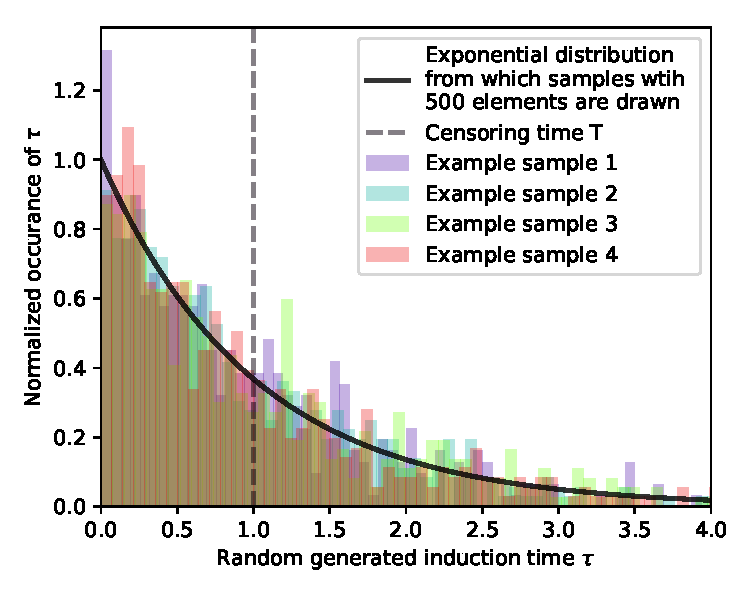
\includegraphics[width = 0.4 \textwidth]{mc_random_sample.pdf}} \hspace{0.5cm}
\subfloat[Distribution of $\hat{\kappa}$ for the previously generated MC samples. The distribution can be described mostly by mean and standard deviation as the number of estimates in the tails are small.]{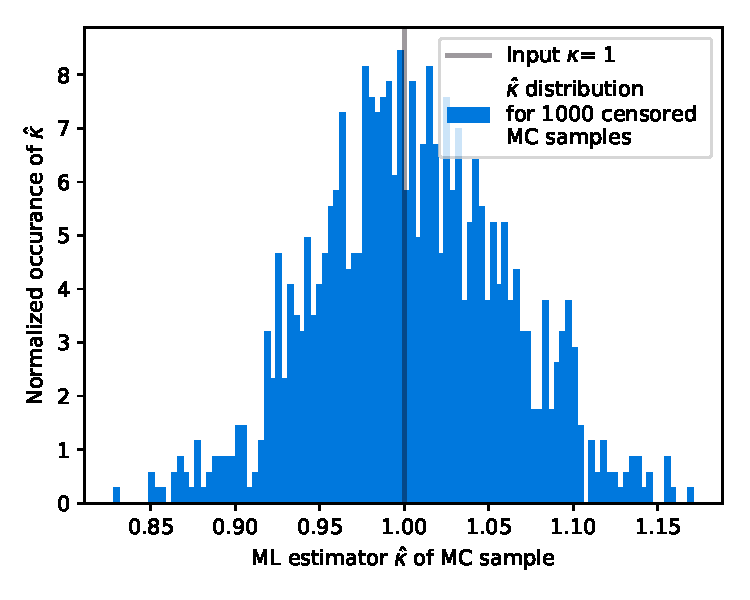
\includegraphics[width = 0.4 \textwidth]{k_estimator_distribution.pdf}}  
\caption{Exemplary samples for a given $\kappa$ as well as the distribution of estimates calculated from the random samples. The uncertainty on $\hat{\kappa}$ is approximated by the standard deviation of the distribution from the corresponding Monte Carlo analysis at a given $\kappa$.}
\label{fig:mc_example}
\end{center}
\end{figure}

Concerning the uncertainty in detail we can ask how long a simulation should be to yield precise results. For this we can first look at the case where $1 \gg \kappa T$ corresponding to a simulation where all boxes showed an nucleation event. In this case we have seen before that $\hat{kappa}^{-1} = \frac{1}{N} \sum_{i=1}^N t_i$. As we assume that the $t_i$ are exponentially distributed we further know that $\sigma_{t} = \kappa^{-1}$. The gaussian error propagation then is given in \autoref{eqn:uncertainty_k_gg}.

\begin{align}
\label{eqn:uncertainty_k_gg}
\frac{\sigma_{\kappa}}{\kappa} &=\frac{1}{\kappa} \sqrt{\sum_{i=1}^N \left( \frac{\partial \kappa}{\partial t_i} \right)^2 \sigma_{t_i}^2 }\\ 
& \; \; \, \vrule
  \begin{aligned}[t]
  \raisebox{0.9cm}{ \makebox[1cm]{}} \text{with }  \frac{\partial \kappa}{\partial t_i} &= \frac{\partial}{\partial t_i} \left( N \left( \sum_{i=1}^N t_i \right)^{-1} \right)\\
  &= -N\left( \sum_{i=1}^N t_i \right)^{-2}  = \frac{\kappa^2}{N} \; \text{,} \\
 \raisebox{-0.4cm}{ \makebox[1cm]{}} \text{and } \sigma_{t} &= \kappa^{-1}
  \end{aligned} \nonumber\\
 &= \frac{1}{\kappa} \sqrt{ N \left( \frac{\kappa^2}{N}\right)^{2} \kappa^{-2} } \\
 &= \frac{1}{\sqrt{N}}
\end{align}
\todo{Is das eine Tautologie!?}

Similarly we can take the limit of $1 \ll \kappa T$ which is the case when the mean nucleation time is much larger than the simulation time and such only a small fraction of the boxes hosted a nucleation event. In this case we can expand the estimator in the fraction of nucleated trajectories $\frac{n}{N}$ to find $\hat{\kappa} \approx \frac{n}{N} \frac{1}{T}$. In this case the decrease of nucleations events due to a smaller amount of available totoal volume is not seen yet, and the only information about the nucleation rate is obtained from the number of boxes with nucleations compared to the number of total amount of boxes used. As $n$ is poission distributed we know that $\sigma_n = \sqrt{n}$. Fixing N and T and using the expectation value of nucleations $n = N \kappa T$ the gaussian error propagation for the relative uncertainty is given in \autoref{eqn:uncertainty_k_ll}.

\begin{align}
\label{eqn:uncertainty_k_ll}
\frac{\sigma_{\kappa}}{\kappa} &= \frac{1}{\kappa} \frac{\sqrt{n}}{NT}\\
&=\frac{\sqrt{N \kappa T}}{N T \kappa}\\
&=\frac{1}{\sqrt{N \kappa T}}
\end{align}

Finally we are also able to not only look at limits analytically, but also to approximate the relative uncertainty directly by means of the aforementioned Monte Carlo method. For this purpose the same procedure as before is used. The number of elements per sample is consistently with the performed simulations taken to be 500 and to archieve good precision the standard deviation of 1000 samples is used for the uncertainty. As can be seen in \autoref{fig:relative_uncertainty} the fluctuations between different evaluations becomes rather small, but increase if using a lower number of samples. To compare the analytically derived limits of the uncertainty with the Monte Carlo results both are drawn into \autoref{fig:relative_uncertainty}.

\begin{figure}[h]
\begin{center}
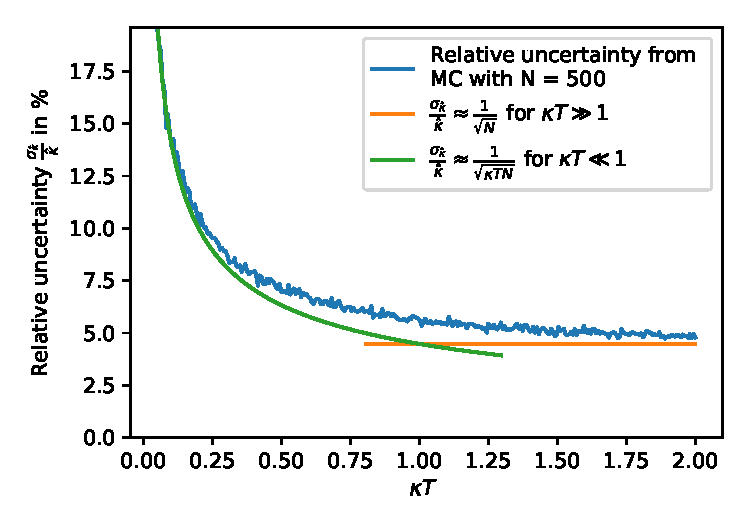
\includegraphics[width = 0.65 \textwidth]{rel_uncertainty_k.pdf}
\caption{Relative uncertainty of the ML estimator for varying $\kappa T$. The x scale is choosen dimensionless such that it indicates the simulation time in comparison to the characteristic nucleation time.}
\label{fig:relative_uncertainty}
\end{center}
\end{figure}

We find that for the limits of $\kappa T \ll 1$ as well as $\kappa T \gg 1$ Monte Carlo results and analytical results are in good accordance while in between the analytical limits only can be used as a rough estimate.\\

What can be seen from \autoref{fig:relative_uncertainty} is that the uncertainty of the estimation drops sharply until about half of the characteristic time, after which it only gains little more precision. This is not surprising as the information is contained in the nucleation times and rather fast many nucleations have occured and the long simulation times add only little of further nucleations. Thus simulating until all boxes had an nucleation event is only necessary if one want s to use the simpler arithmetic mean of the induction times as a characteristic time, or if any oher constraints make it necessary to reach nucleation of all boxes.

\section{Nucleation rate comparison}
\label{sec:nucleation_rates}
Finally we are able to evaluate the induction time distribution to find 


All Nucleation rates that can be found.-> mayhap ask Hajo.\\
-nucleation rates without\\
-nucleation rates with small particles\\


\section{Memory Kernels}
\label{sec:memory_kernels}
Memory kernels of systems at various densities. Depends strongly on what is found here\\
-memory kernels of 16k system at varying points of time\\
-memory kernels from fall article\\
-maybe memory kernels of 1m system, but do not know what to say. Maybe only mention that after seeing the 16k system to have only memory kernes at about middle of the time, no true memory kernel is visible in the 1m system as volume fractions have been to low with to large calculation times.\\
 

\newpage

\chapter{Conclusion - Summary}
% !TEX root = writing_version.tex

%\section{Conclusion}
\label{sec:conclusion}

\begin{description}
\item[summary]
\item[key results]
\item[future outlook]
\end{description}

\newpage

\pagestyle{plain}
\renewcommand{\chapterpagestyle}{plain}
\chapter{Appendix}
% !TEX root = writing_version.tex

\appendix
\section{appendix a}
\label{sec:appendix}

\newpage

\printbibliography

\end{document}







